\documentclass[9pt]{beamer}
\usepackage{slide}

\begin{document}
\title{\textbf{Optimizing AoII with IoT Sensor Reading Dataset}}
\author{\textbf{Thanh LE}}
\institute{Supervisor: Yusheng Ji, John C.S. Lui, Hong-Linh Truong}
\date{\today}
\titlegraphic{
  
\includegraphics[width=2cm]{figure/title/sokendai.png}\hspace{1cm}
  
\includegraphics[width=1cm]{figure/title/nii.png}\hspace{1cm}
  
\includegraphics[width=1cm]{figure/title/aalto.png}
}
\maketitle
\begin{frame}
    \frametitle{Agenda}
    \tableofcontents
\end{frame}

\section{Introduction}

\begin{frame}{Background}
    \begin{figure}
        \centering
        \animategraphics[autoplay,loop,width=0.9\linewidth]{12}{figure/intro/motivation/frame_}{000}{10}
        \caption{The number of IoT applications are increasing.}
    \end{figure}
\end{frame}

\begin{frame}{Motivation + Challenge + Contribution}
    \begin{columns}
        \begin{column}{0.48\textwidth}
            \begin{block}{Background}
                \begin{itemize}
                    \item \alert{Increase} number of IoT \alert{applications}
                    \item \alert{Massive} number of low-power \alert{sensors} generating data sporadically
                    \item \alert{Limited} wireless resources
                \end{itemize}
                $\rightarrow$ develop new \alert{data sampling policy}
            \end{block}
        \end{column}
        \begin{column}{0.48\textwidth}
            \begin{block}{Challenge}
                Previous works tested their protocols on
                \begin{itemize}
                    \item Saturated traffic (not IoT)
                    \item Probabilistic traffic models based on two-state Markov Models
                    \item Slowly varying time-series $\rightarrow$ less traffic demand
                \end{itemize}
            \end{block}
        \end{column}
    \end{columns}
    \begin{block}{Contribution}
        \begin{itemize}
            \item Test on AaltoSEA's \alert{realistic IoT dataset} (faster fluctuation in data $rightarrow$ more demand)
            \item Measure \alert{end-to-end performance} on modern grant-free random access (\gls{irsa} model)
            \item Propose \gls{xab} for \alert{online batch learning} to select best sampling rate
            \item Minimize \alert{\gls{aoii}} while sending data \alert{conservatively}
        \end{itemize}
    \end{block}
\end{frame}

\section{Related Works}

\begin{frame}{Related works - Remote Estimation}
    \begin{block}{Variation-aware Sampling}
        \begin{itemize}
            \item \fullcite{kim2020user}
            \item Propose a \alert{variation-aware} sampling scheme to reduce communication resource consumption while maintaining a small mean value error
            \item Tested on temperature and water quality datasets with a granularity of \alert{10 minutes to 1 hour}.
        \end{itemize}
    \end{block}
    \begin{block}{\gls{aoii}}
        \begin{itemize}
            \item \fullcite{maatouk2022age}
            \item Introduce the \gls{aoii} metric, which merges \alert{value error} and \alert{timeliness} into a single measure
            \item Propose an optimal policy based on \alert{stable} state transition probabilities
            \item State transition probabilities fluctuate $\rightarrow$ computationally intensive to adapt
        \end{itemize}
    \end{block}
\end{frame}

\begin{frame}{Related works - Remote Estimation}
    \begin{block}{SAC minimize \gls{aoii} under changing dynamics}
        \begin{itemize}
            \item \fullcite{tong2023semantic}
            \item Tested on the Intel Berkeley dataset with \alert{slowly varying} temperature and humidity data
            \item Using DNN on IoT devices (\alert{computationally complexity problem})
            \item Require \alert{frequent acknowledgements}
        \end{itemize}
    \end{block}
    \begin{block}{Age of Event}
        \begin{itemize}
            \item \fullcite{huang2025minimizing}
            \item Introduce the \gls{aoe} metric (extend of \gls{aoii})
            \item Utilizing a dataset characterized by \alert{sparse events} over a \alert{wide area} (LA-USA)
        \end{itemize}
    \end{block}
\end{frame}

\begin{frame}{Related works - Remote Estimation}
    \begin{block}{Minimize AoI under IRSA Transmission Model}
        \begin{itemize}
            \item \fullcite{munari2021modern}
        \end{itemize}
    \end{block}
    \begin{block}{Without feedback}
        \begin{itemize}
            \item \fullcite{munari2024monitoring}
            \item Propose \alert{reactive}, \alert{maximize throughput}, and \alert{hybrid} policy
            \item Tested on \alert{statistical traffic model}
            \item \alert{No acknowledgement} feedback
        \end{itemize}
    \end{block}
\end{frame}

\begin{frame}{Related works - IoT Dataset}
    \begin{block}{IoT Dataset}
        \begin{itemize}
            \item \texttt{Berkeley}: \fullcite{intellabdata}
            \item \texttt{BTS sensors}: \fullcite{truong2022haivan}
            \item \texttt{Toy factory}: \fullcite{nguyen2024security}
        \end{itemize}
    \end{block}
\end{frame}

\begin{frame}{Contribution - recap}
    \begin{block}{Contribution}
        \begin{itemize}
            \item Test on AaltoSEA's \alert{realistic IoT dataset} (faster fluctuation in data $rightarrow$ more demand)
            \item Measure \alert{end-to-end performance} on modern grant-free random access (\gls{irsa} model)
            \item Propose \gls{xab} for \alert{online batch learning} to select best sampling rate
            \item Minimize \alert{\gls{aoii}} while sending data \alert{conservatively}
        \end{itemize}
    \end{block}
\end{frame}

% \begin{frame}{a more recent paper for dataset}
%     \begin{columns}
%         \begin{column}{0.48\textwidth}
%             \begin{figure}
%                 \centering
%                 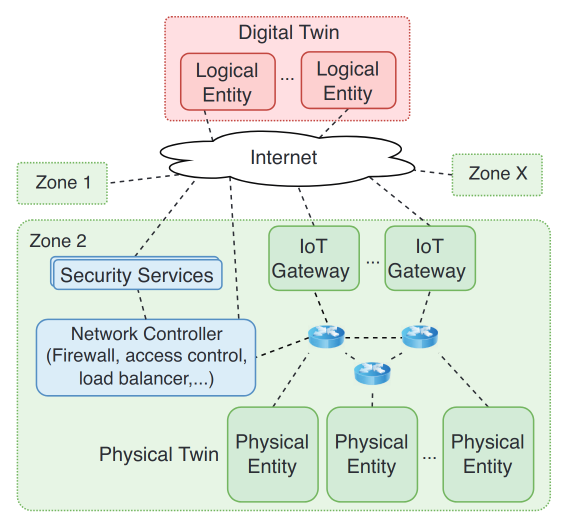
\includegraphics[width=\linewidth]{figure/related/sindit.png}
%                 \caption{Overview of a common deployment model for digital twin in manufacturing}
%             \end{figure}
%         \end{column}
%         \begin{column}{0.48\textwidth}
%             \begin{block}{Simulation model}
%                 \begin{itemize}
%                     \item SINDIT, a Digital Twin of the Fischertechnik Training Factory
%                     \item 37 sensorss
%                     \item Constantly send sensor data to the digital twin
%                     \item Mininet network simulation
%                 \end{itemize}
%             \end{block}
%             \begin{figure}
%                 \centering
%                 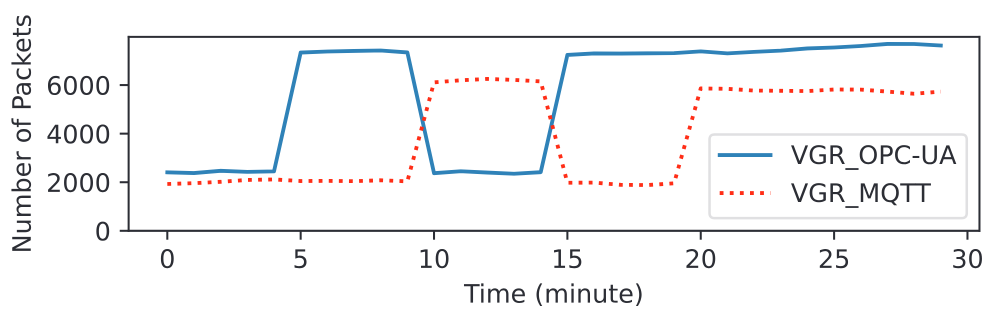
\includegraphics[width=\linewidth]{figure/related/vgr.png}
%                 \caption{Network packets from VGR (vision guided robot) to the two gateways.}
%             \end{figure}
%         \end{column}
%     \end{columns}
%     \footfullcite{nguyen2024security}
% \end{frame}
%
% \begin{frame}{AoII DT}
%     \begin{block}{System model}
%         \begin{figure}
%             \centering
%             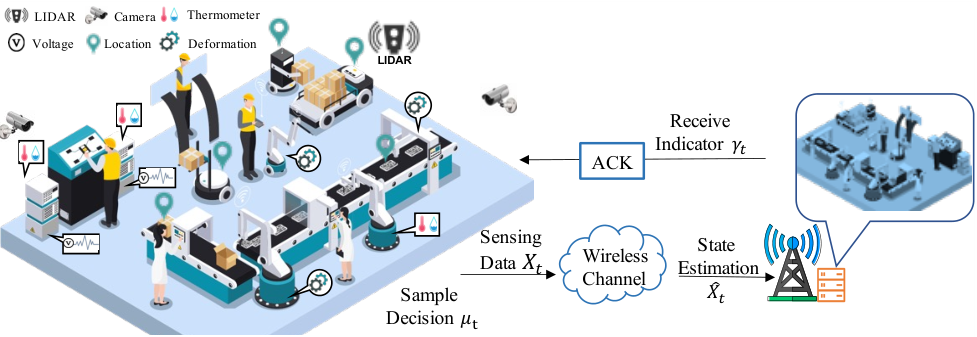
\includegraphics[width=\linewidth]{figure/related/aoii-dt.png}
%             \caption{Remote state estimation system in a digital twin empowered smart factory.}
%         \end{figure}
%     \end{block}
%     \footfullcite{tong2023semantic}
% \end{frame}
%
% \begin{frame}{AoII DT}
%     \begin{columns}
%         \begin{column}{0.48\textwidth}
%             \begin{block}{Mechanism}
%                 \begin{itemize}
%                     \item SAC for CMDP
%                     \item Agent: device
%                     \item Action: sample and transmit or stay idle
%                     \item Observation: AoI at the server, estimation error, and the data reception indicator
%                     \item Cost: communication budget is limited
%                     \item Reward: minus AoII
%                 \end{itemize}
%             \end{block}
%         \end{column}
%         \begin{column}{0.48\textwidth}
%             \begin{block}{Cons}
%                 \begin{itemize}
%                     \item Sensor dataset: Intel Berkeley research lab (2004)
%                     \item Single access point
%                 \end{itemize}
%             \end{block}
%         \end{column}
%     \end{columns}
%     \footfullcite{tong2023semantic}
% \end{frame}
%
% \begin{frame}{IN-XS}
%     \begin{columns}
%         \column{.58\textwidth}
% 	\begin{block}{What are \gls{inxs}?}
%                 \begin{itemize}
%                     \item Short-range
%                     \item Low-power
%                     \item Handle extreme communication requirements
%                         \begin{itemize}
%                             \item Ultra-reliable
%                             \item Low-latency
%                             \item Heavy-interference
%                         \end{itemize}
%                 \end{itemize}
%             \end{block}
%         \column{.38\textwidth}
%             \begin{block}{Applications}
%                 \begin{itemize}
%                     \item Industrial control
%                     \item Autonomous vehicle
%                     \item Smart healthcare
%                 \end{itemize}
%             \end{block}
%     \end{columns}
%     \begin{figure}
%         \centering
%         \begin{subfigure}[b]{0.54\linewidth}
%             \centering
%             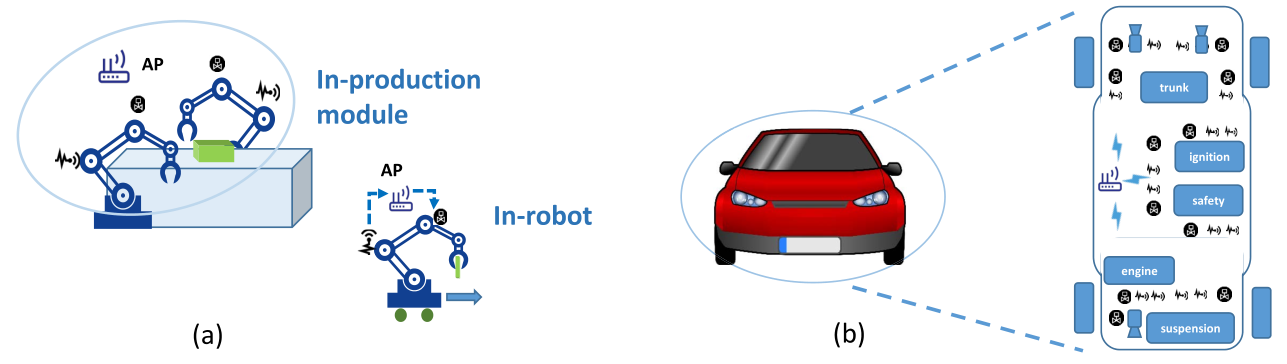
\includegraphics[width=\linewidth]{figure/related/installations_1.png}
%         \end{subfigure}
%         \hfill
%         \begin{subfigure}[b]{0.44\linewidth}
%             \centering
%             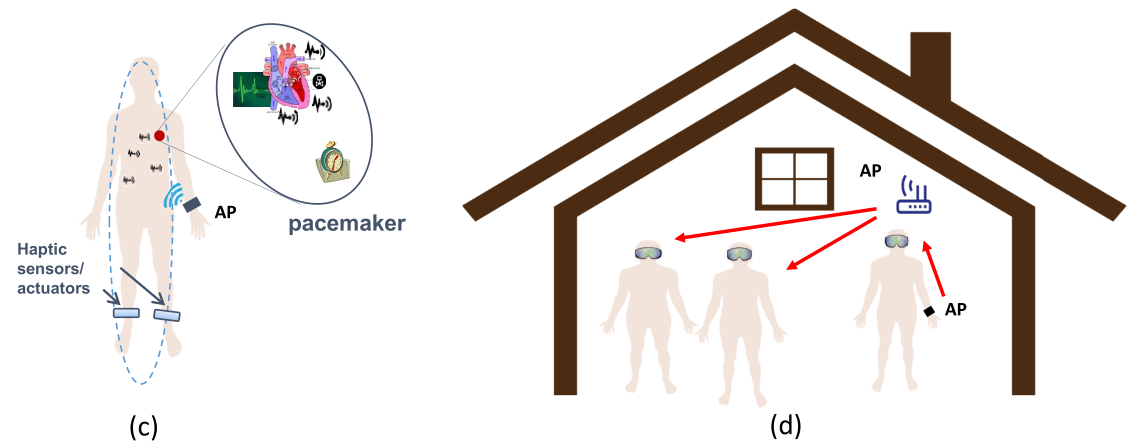
\includegraphics[width=\linewidth]{figure/related/installations_2.png}
%         \end{subfigure}
%         \caption{Examples of installations for (a) \alert{in}-dustrial, (b) \alert{in}-vehicle, (c) \alert{in}-body and (d) \alert{in}-house subnetworks.}
%     \end{figure}
%     \footfullcite{adeogun2022multi}
% \end{frame}

\section{System Model and Problem Formulation}

\begin{frame}{System Model Overview}
    \begin{figure}
        \centering
        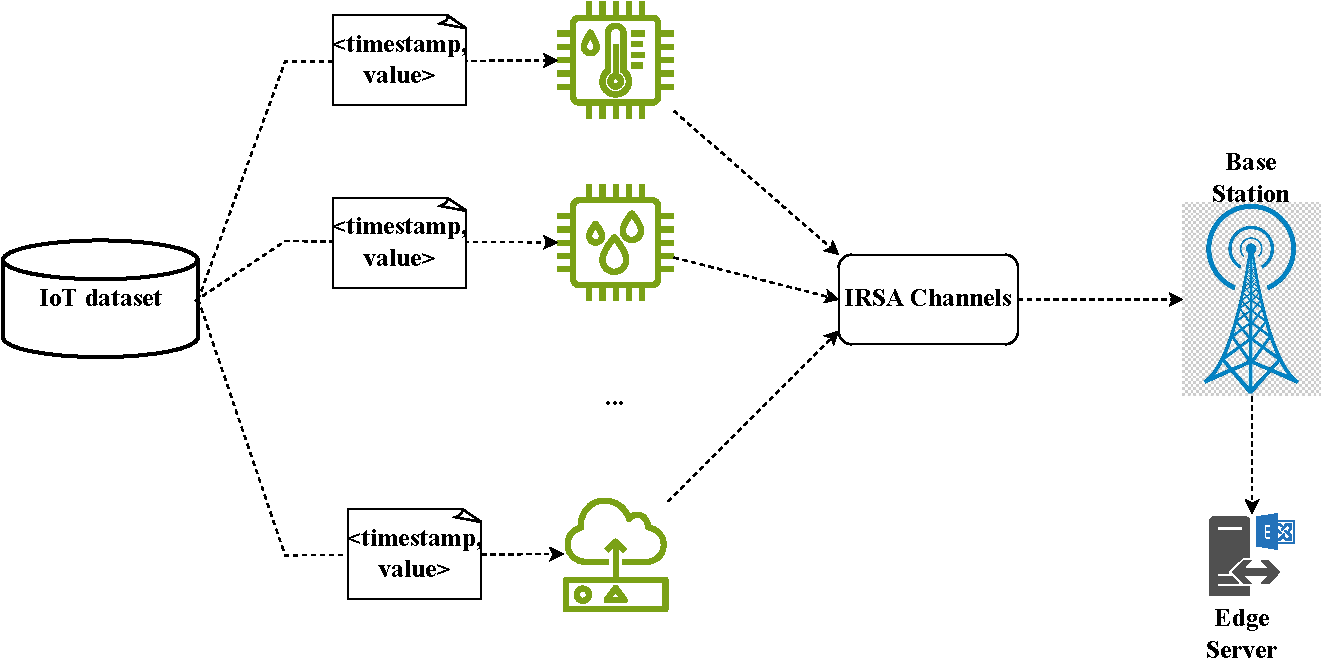
\includegraphics[width=\linewidth]{figure/system/system-model.pdf}
        \caption{Overview of our system model}
    \end{figure}
\end{frame}

% \begin{frame}{Transmission model: IRSA}
%     \begin{figure}
%         \centering
%         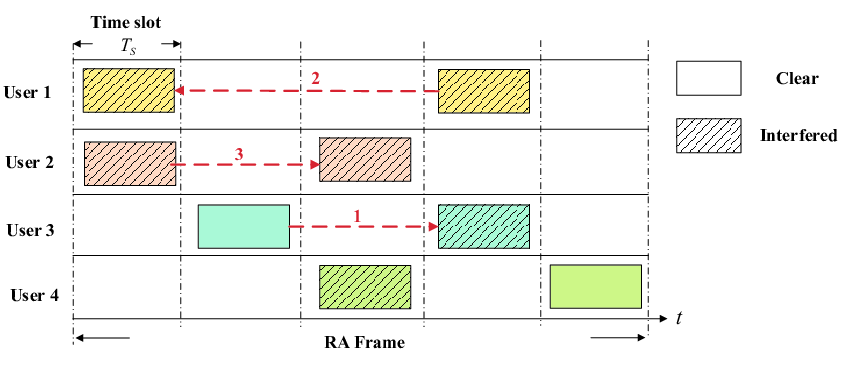
\includegraphics[width=\linewidth]{figure/system/irsa.png}
%         \caption{Example of \gls{irsa} transmission model}
%     \end{figure}
% \end{frame}

% \begin{frame}{Performance Metric: AoII}
%     \begin{figure}
%         \centering
%         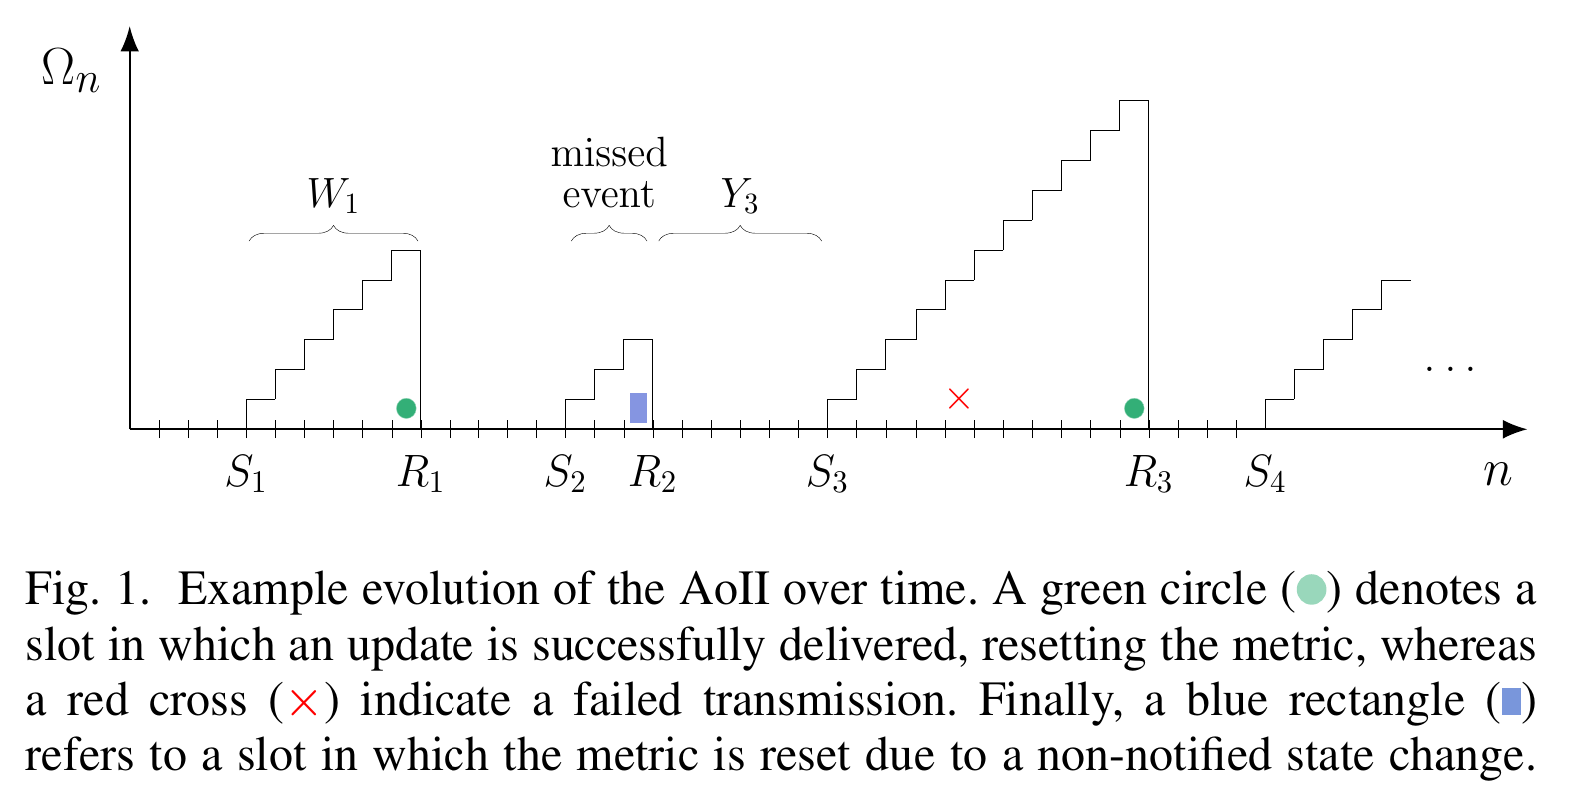
\includegraphics[width=\linewidth]{figure/system/aoii.png}
%         \caption{Example of \gls{aoii} performance metric}
%     \end{figure}
% \end{frame}

\begin{frame}{System Model}
    \begin{columns}
        \begin{column}{0.48\textwidth}
            \begin{block}{Network Model}
                \begin{itemize}
                    \item A single \gls{bs}
                    \item $K$ devices
                    \item $M$ grant-free random access resource blocks (channels)
                    \item Uplink data, short packet communication
                    \item In average, send $L$ repetition of a packet
                    \item Slotted time $n$
                \end{itemize}
            \end{block}
        \end{column}
        \begin{column}{0.48\textwidth}
            \begin{block}{Transmission Model}
                \begin{itemize}
                    \item \gls{irsa} collision resolution
                    \item Devices send $L$ repetition of a packet in average
                    \item $L < M$
                    \item No immediate ACK/NACK
                    \item Each round $t$, exists $N$ uplink transmission time slot before a feedback message
                \end{itemize}
            \end{block}
        \end{column}
    \end{columns}
\end{frame}

\begin{frame}{Performance Metric}
    \begin{block}{\gls{aoii}}
        \begin{equation}
            \Omega_k(n) = \delta_k(n) (n - S_k(n))
        \end{equation}
        where
        \begin{itemize}
            \item $\Omega_k(n)$: \gls{aoii} of device $k$ at time slot $n$
            \item $\delta_k(n) := |X_k(n) - \hat{X}_k(n)| \mathbbm1\{|X_k(n) - \hat{X}_k(n)| \ge \epsilon \}$: estimation error of device $k$ at time slot $n$
            \item $S_k(n) := \text{max} \{S_k^i | S_k^i \le n \}$: the last time slot at which the receiver started having an erroneous estimate ($|X_k(n) - \hat{X}_k(n)| \ge \epsilon$)
        \end{itemize}
    \end{block}
\end{frame}

% \begin{frame}{Prof. Stephan Sigg's Team}
%     \begin{figure}
%         \centering
%         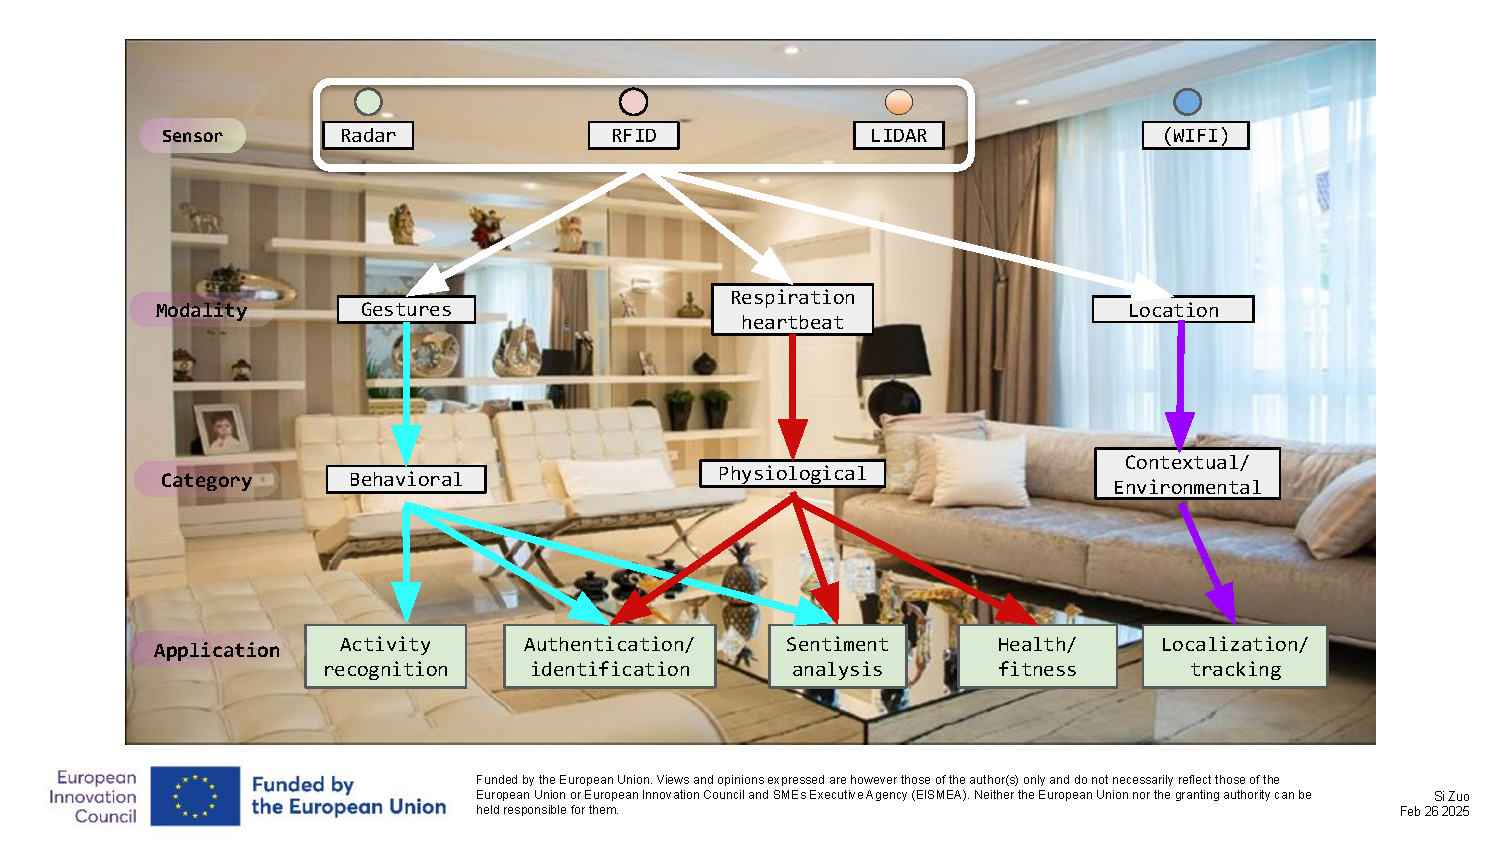
\includegraphics[width=\linewidth]{figure/system/si_zuo.pdf}
%     \end{figure}
% \end{frame}
%
% \begin{frame}{Prof. Stephan Sigg's Team}
%     \begin{columns}
%         \begin{column}{0.48\textwidth}
%             \begin{figure}
%                 \centering
%                 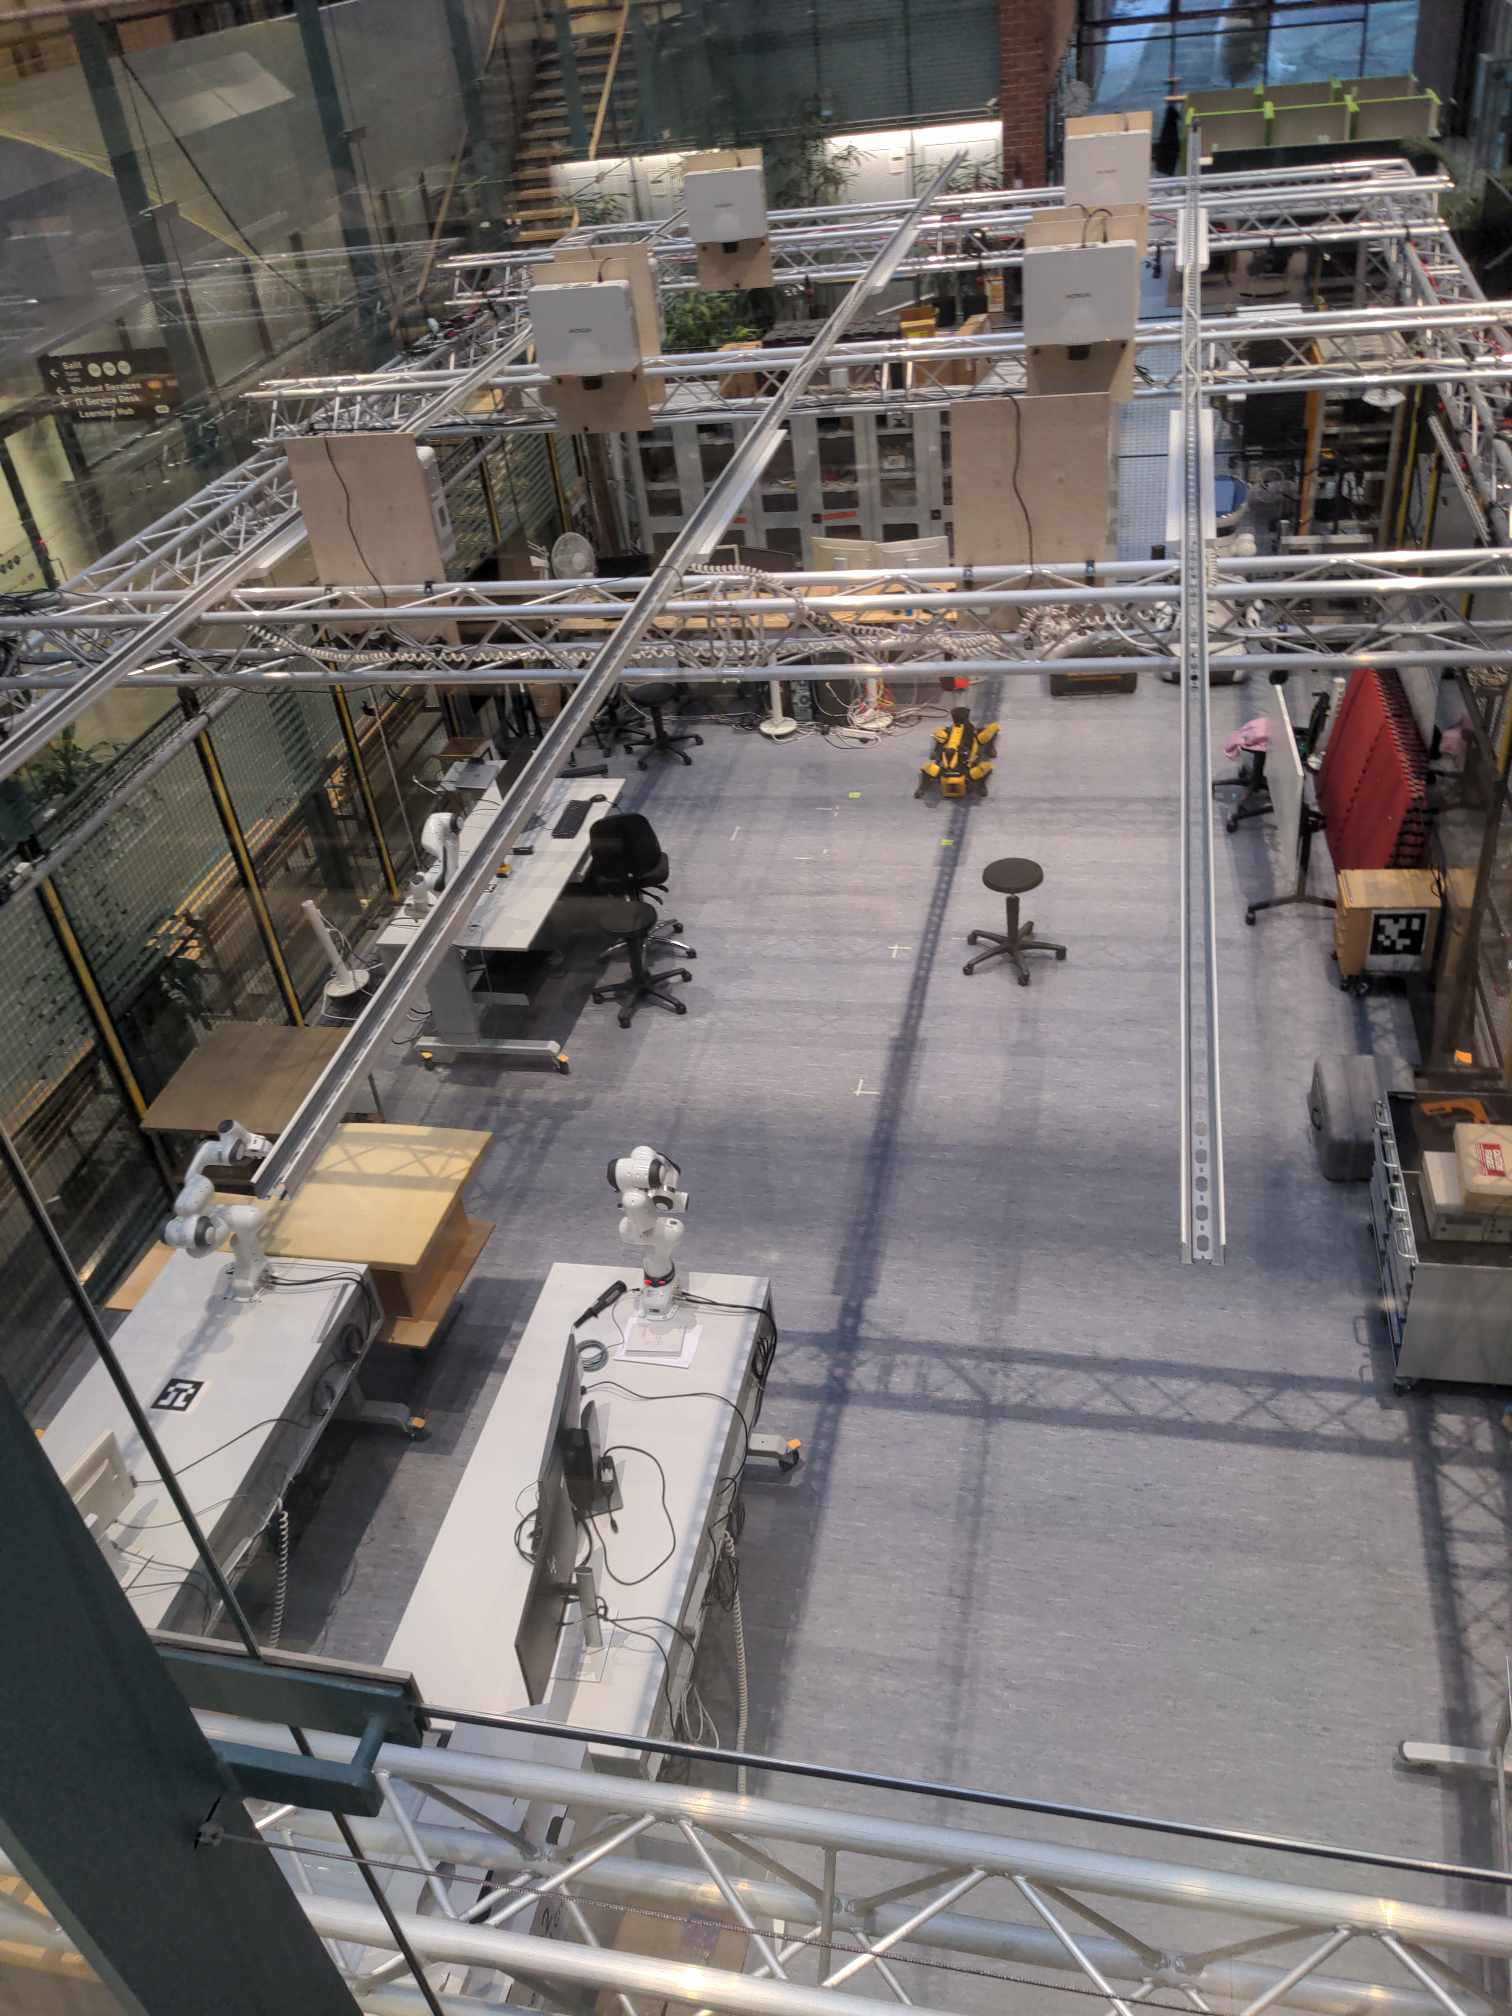
\includegraphics[width=0.8\linewidth]{figure/system/lab.jpg}
%                 \caption{Electrical engineering lab}
%             \end{figure}
%         \end{column}
%         \begin{column}{0.48\textwidth}
%             \begin{figure}
%                 \centering
%                 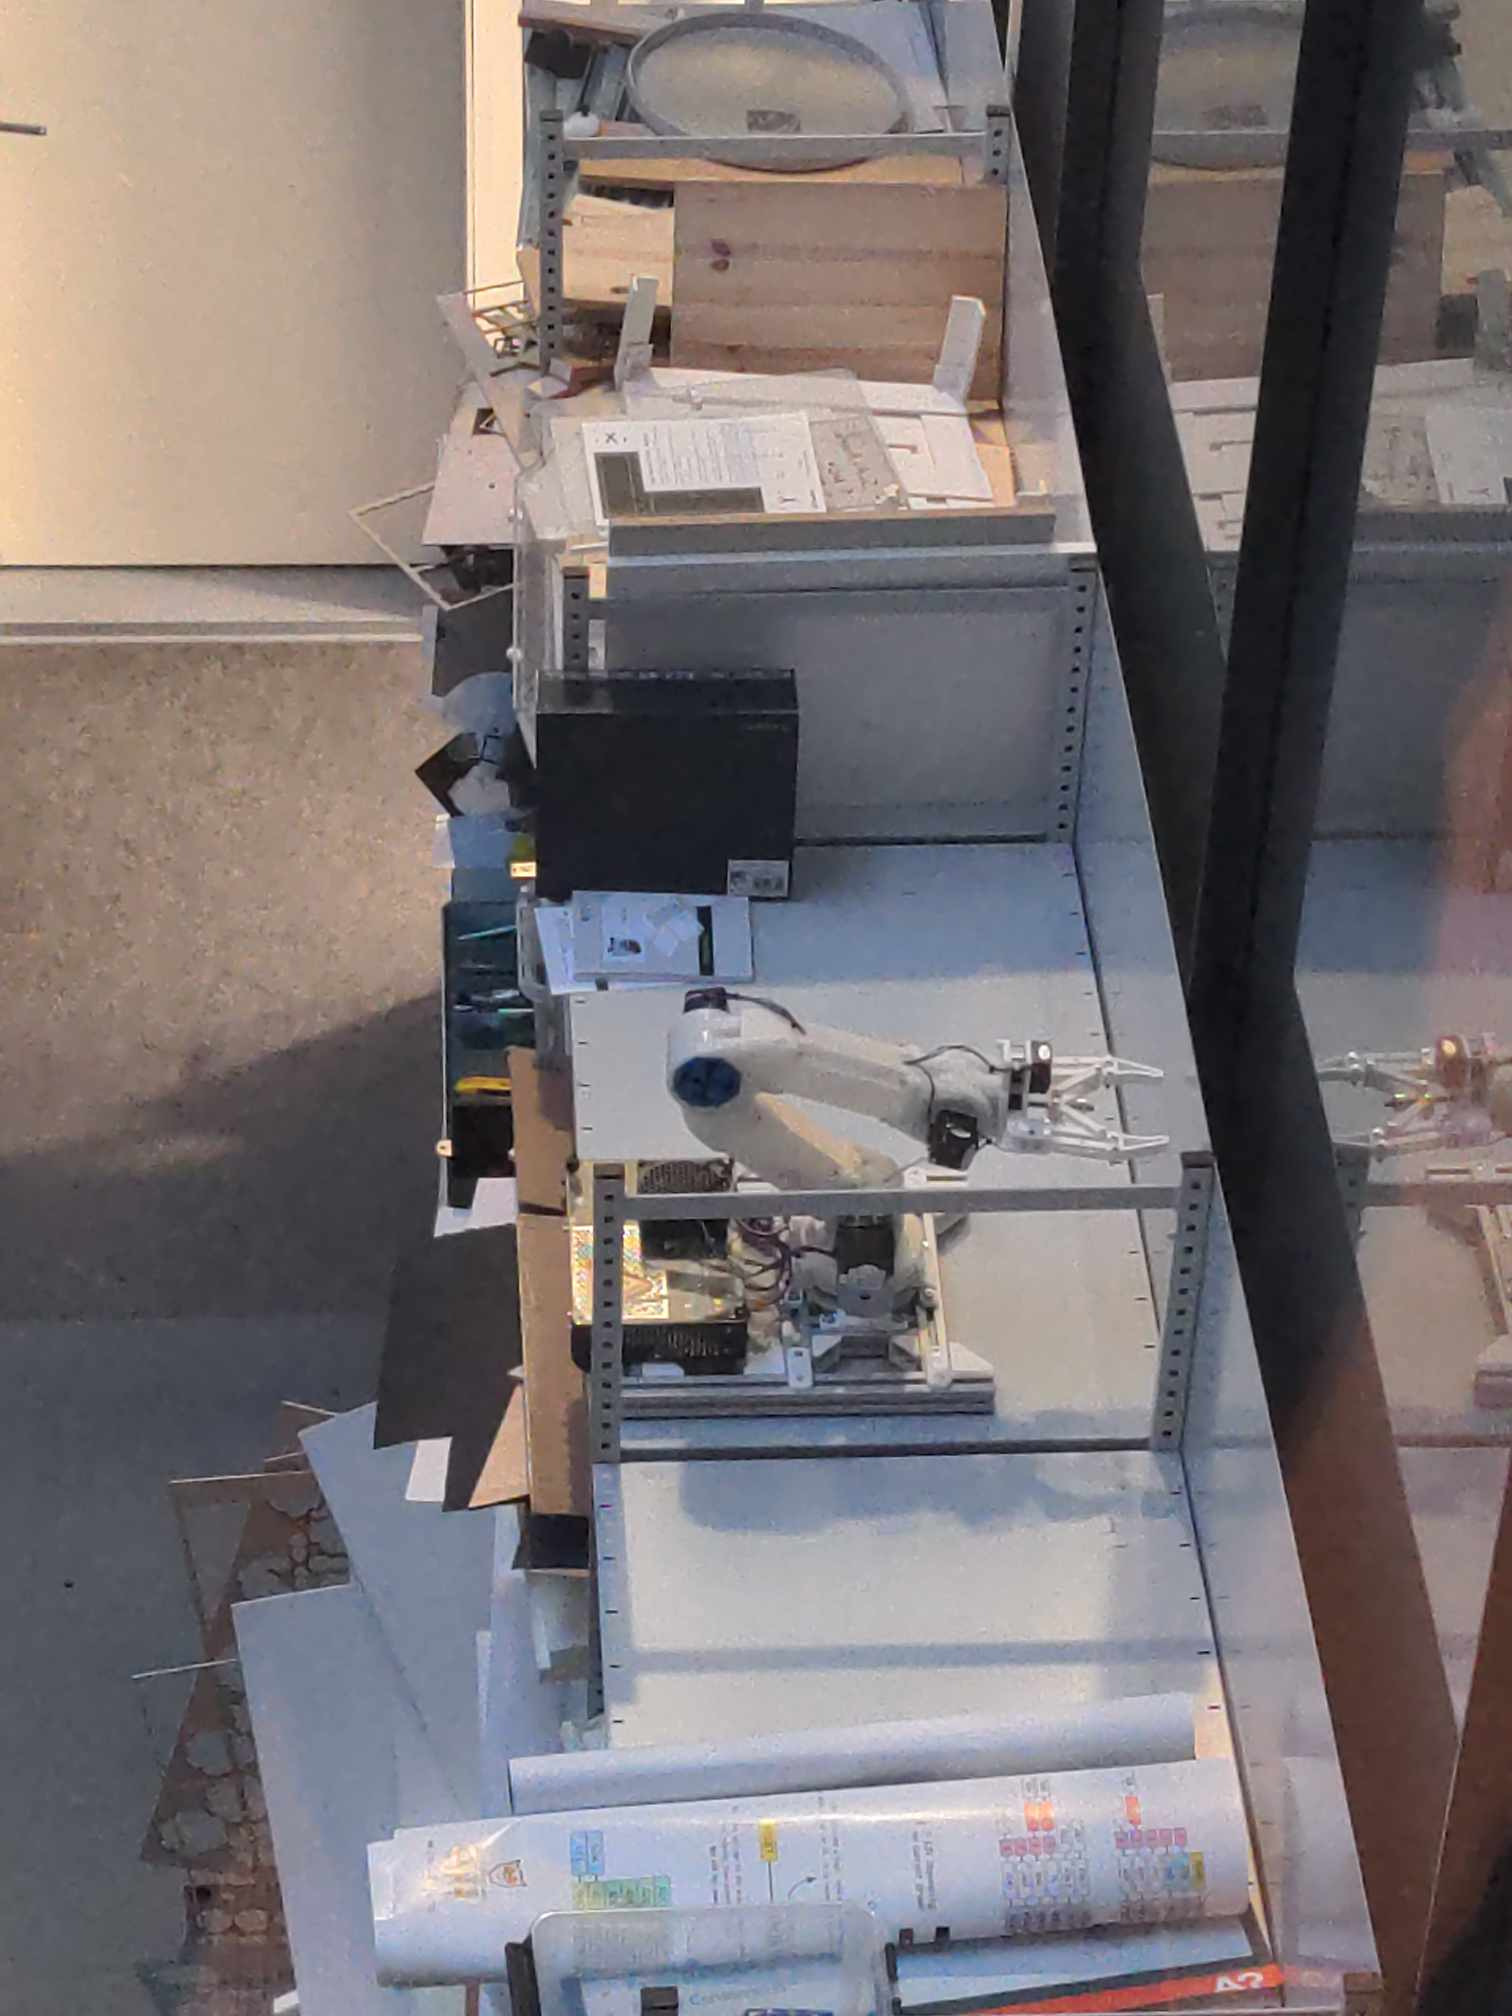
\includegraphics[width=0.8\linewidth]{figure/system/robot_arm.jpg}
%                 \caption{Robot arm}
%             \end{figure}
%         \end{column}
%     \end{columns}
% \end{frame}




% \begin{frame}{System Model}
%     \framesubtitle{Network Model}
%     \begin{columns}
%         \column{.58\textwidth}
%             \begin{figure}
%                 \centering
%                 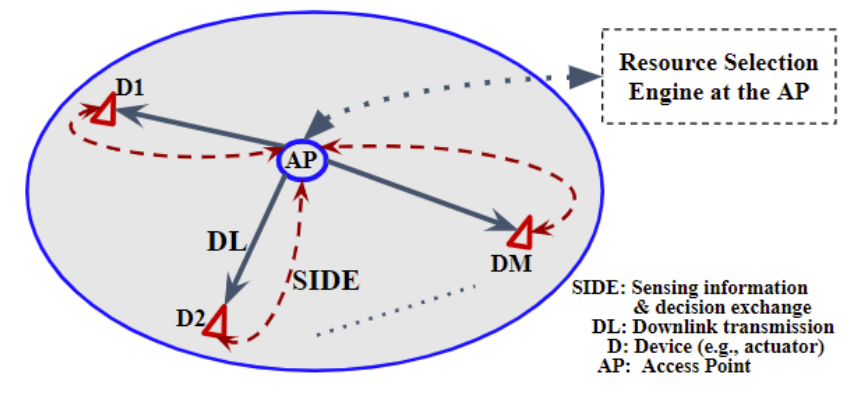
\includegraphics[width=0.99\linewidth]{figure/system/system-model.png}
%                 \caption{System model of \gls{inxs} networks}
%             \end{figure}
%         \column{.38\textwidth}
%             \begin{figure}
%                 \centering
%                 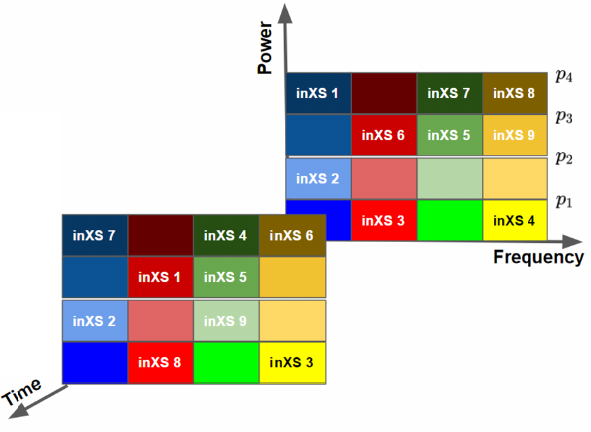
\includegraphics[width=0.99\linewidth]{figure/system/wireless-resource.png}
%                 \caption{System model of \gls{inxs} networks}
%             \end{figure}
%     \end{columns}
%     \begin{columns}
%         \column{.58\textwidth}
%             \begin{block}{Network Model}
%                 \begin{itemize}
%                     \item An \gls{ap}: manage all subnetworks
%                     \item $N$: number of subnetworks
%                     \item $M_n$: number of devices in the $n^{th}$ subnetwork
%                 \end{itemize}
%             \end{block}
%         \column{.38\textwidth}
%             \begin{block}{Wireless Resources}
%                 \begin{itemize}
%                     \item $K$: number of shared frequency channels
%                     \item $Z$: number of discrete power levels
%                 \end{itemize}
%             \end{block}
%     \end{columns}
% \end{frame}
%
% \begin{frame}{System Model}
%     \framesubtitle{Channel Model}
%     \begin{columns}
%         \column{.38\textwidth}
%             \begin{block}{Path Loss}
%                 \begin{equation}
%                     L_{AB} = \frac{{}c^2d^{-\alpha}_{AB}}{16\pi^2f^2}
%                 \end{equation}
%                 \begin{itemize}
%                     \item $d_{AB}$: Distance from node $A$ to node $B$.
%                     \item $c$: Speed of light.
%                     \item $\alpha$: Path-loss exponent.
%                     \item $f$: Carrier frequency.
%                 \end{itemize}
%             \end{block}
%         \column{.58\textwidth}
%             \begin{block}{Shadowing}
%                 \begin{equation}
%                     X_{AB} = \ln\left\{\frac{1-e^{\left(-\frac{d_{AB}}{d_c}\right)}}{\sqrt{2}\sqrt{1+e^{\left(-\frac{d_{AB}}{d_c}\right)}}}(\mathbf{S}(A) + \mathbf{S}(B))\right\}
%                 \end{equation}
%                 \begin{itemize}
%                     \item $d_c$: Correlation distance.
%                     \item $\mathbf{S}(A)$, $\mathbf{S}(B)$: Covariance functions.
%                 \end{itemize}
%             \end{block}
%     \end{columns}
%
%     \begin{block}{Received (interference) power}
%         \begin{equation}
%             P_{AB}(\kappa_A(t)) = \kappa_A(t)L_{AB}(t)X_{AB}(t)|h_{AB}(t)|^2
%         \end{equation}
%         \vspace{-.5cm}
%         \begin{itemize}
%             \item $\kappa_A(t)$: Transmit power of node $A$.
%             \item $h_{AB}(t)$: Rayleigh distributed small-scale fading factor
%         \end{itemize}
%     \end{block}
% \end{frame}
%
% \begin{frame}{System Model}
%     \framesubtitle{Rate Expression}
%         \begin{block}{\gls{sinr}}
%             \begin{itemize}
%                 \item Assuming at time $t$, the subnetwork $n$ operates over the channel $c_k$
%                 \item The \gls{sinr} from device $m$ can be expressed as:
%                     \begin{equation}
%                         \gamma_{nm}(c_k,\boldsymbol{\kappa}^k(t)) = \frac{P_{nm}(c_k,\kappa^k_n(t))}{\sum_{i\in\mathcal{I}_k(t)}{P_{ni}(c_k,\kappa^k_i(t)) + \boldsymbol{\sigma}^2_{nm}(t)}}
%                     \end{equation}
%                     \begin{itemize}
%                         \item ${P_{nm}(c_k,\kappa^k_n(t))}$: received signal power in $n$-th inXS.
%                         \item $\mathcal{I}_k(t)$: set of interfering devices.
%                         \item $\sigma^2_{nm}(t)$: noise power.
%                     \end{itemize}
%             \end{itemize}
%         \end{block}
%         \begin{block}{Achieved Capacity}
%             \begin{itemize}
%                 \item Rely on the Shannon approximation, the achieved capacity can be written as:
%                 \begin{equation}
%                     \zeta_{nm}(c_k,t) \approx W_k \log_2{(1+\gamma_{nm}(c_k,\boldsymbol{\kappa}^k(t)))}
%                 \end{equation}
%                 \vspace{-.5cm}
%                 \begin{itemize}
%                     \item $W_k$: Bandwidth of channel $c_k$.
%                 \end{itemize}
%             \end{itemize}
%         \end{block}
% \end{frame}

% \section{Problem Formulation}

\begin{frame}{Problem Formulation}
    \begin{block}{Optimize Randomized Sampling Rate - Minimize \gls{aoii} and \gls{irsa} channel utilization}
        \begin{equation}
            \underset{x_k \in [0, \overline{x}]}{\text{minimize}} \; \sum_{t=1}^T \Big[ \sum_{n=1}^{N} \Omega_k(n) \Big] + \alpha u_k(t)
        \end{equation}
        where
        \begin{itemize}
            \item $x_k$: randomized transmission probability
            \item $\overline{x}$: tranmission probability s.t. if every devices transmit with probability $\overline{x}$, the throughput of \gls{irsa} channels are maximized
            \item $u_k(t)$: utilization of device $k$ at round $t$, count total number of packet sent per round
        \end{itemize}
    \end{block}
%     \begin{block}{Objective 1}
%         \begin{itemize}
%             \item Select randomized sampling probability
%             \item Minimize \gls{aoii}
%         \end{itemize}
%     \end{block}
%     \begin{block}{Objective 2}
%         \begin{itemize}
%             \item Select randomized sampling probability
%             \item Minimize \gls{irsa} channel utilization
%         \end{itemize}
%     \end{block}
\end{frame}

\section{Propose Method}

\begin{frame}{Multi-player X-armed Bandits Formulation}
    \begin{block}{Player}
        \begin{itemize}
            \item A device $k$ is a player
            \item Independently select their randomized uplink transmission probability
        \end{itemize}
    \end{block}
    \begin{block}{Continuous arms}
        \begin{itemize}
            \item A player $k$ chooses a continuous arm $x_k \in [0, \overline{x}]$
        \end{itemize}
    \end{block}
    \begin{block}{Reward}
        \begin{itemize}
            \item Reward of a player $k$
                \begin{equation}
                    r_k(x_k, t) = - \Big[ \frac{1}{N} \sum_{n=1}^{N} \Omega_k(n) \Big] - \alpha u_k(x_k, t)
                \end{equation}
        \end{itemize}
    \end{block}
\end{frame}

\begin{frame}{X-armed Bandits Algorithm}
    \begin{block}{Hierarchical Partitioning}
        \begin{itemize}
            \item Discretize search space $\mathcal{X} = [0, \overline{x}]$ into nodes
            \item Denotes the partitioning $\mathcal{P}_{h, i}$
            \item $h$ is the depth of the partition
            \item $i$ is node index
            \item A node $\mathcal{P}_{h, i}$ can be separated into two child nodes: $\mathcal{P}_{h+1, 2i}$ and $\mathcal{P}_{h+1, 2i+1}$
            \item Traverse the partitions and selecting nodes with higher rewards to split $\rightarrow$ get higher precision solution
        \end{itemize}
    \end{block}
\end{frame}

\begin{frame}{X-armed Bandits Algorithm}
    \begin{block}{Resolution Descriptor}
        \begin{itemize}
            \item Let $OE_h$ to be the \alert{resolution} of level $h$
            \item $OE_h$ is a function that bounds the change of $f$ around its global optimum within domain $\mathcal{P}_{h, i^*_h}$
                \begin{equation}
                    \forall h \ge 0, \forall x \in \mathcal{P}_{h, i^*_h}, f(x) \ge f(x^*) - OE_h
                \end{equation}
            \item $\mathcal{P}_{h, i^*_h}$ is the node on depth $h$ that contain the global optimum $x^*$
        \end{itemize}
    \end{block}
    \begin{block}{Uncertainty Quantifier}
        \begin{itemize}
            \item Let $SE_{h, i}$ to be the \alert{uncertainty estimate} for node $\mathcal{P}_{h, i}$
            \item \gls{vhct}: estimate $SE$ adaptively
        \end{itemize}
    \end{block}
    \begin{block}{Arms extension}
        \begin{itemize}
            \item Continuously search nodes from root to leaves
            \item Until finding $OE_h < SE_{h, i}$ then pull node $i$
            \item Complete sampling a node when $OE_h \ge SE_{h, i}$
            \item Split best completed node in each depth $h$
        \end{itemize}
    \end{block}
\end{frame}

\begin{frame}{X-armed Bandits Regret Bound}
    \begin{block}{General Local Smoothness (GLS) Condition}
        \begin{equation}
            \forall h \ge 0, \forall x \in \mathcal{P}_{h, i^*_h}, f(x) \ge f(x^*) - \nu \rho^h
        \end{equation}
        where $\nu > 0$, $\rho \in (0, 1)$, and $OE_h = \nu \rho^h$
    \end{block}
    \begin{block}{Theorem: regret bound of VHCT}
        Assume that reward function $f$ satisfies GLS condition, then the expected cumulative regret of \gls{vhct} is upper bounded by
        \begin{equation}
            \mathbb{E}[R_n^{\text{VHCT}}] \le 2 \sqrt{2n\log(4n^3)} +
                                              C_1 V_{\text{max}} ^ {\frac{1}{d + 2}} n^{\frac{d+1}{d+2}} \log(n)^{\frac{1}{d+2}} +
                                              C_2 n^{\frac{2d+1}{2d+4}} \log(n)
        \end{equation}
        where
        \begin{itemize}
            \item $V_{\text{max}}$: maximum variance of $SE_{h, i}$
            \item $C_1, C_2$ are constants
            \item $d$ is the number of nodes $\mathcal{P}_{h, i}$ to achieve near optimal solution (depend on $\nu$ and $\rho$)
        \end{itemize}
    \end{block}
\end{frame}

\begin{frame}{Tight Resolution Descriptor (our contribution)}
    \begin{block}{Recall that}
        $OE_h$ is a function that bounds the change of $f$ around its global optimum within domain $\mathcal{P}_{h, i^*_h}$
            \begin{equation}
                \forall h \ge 0, \forall x \in \mathcal{P}_{h, i^*_h}, f(x) \ge f(x^*) - OE_h,
            \end{equation}
        and $OE_h = \nu \rho^h$
        $\rightarrow$ select tighter $\nu \rho^h$ reduce number of nodes to achieve near optimal solution $d$
    \end{block}
    \begin{block}{Reward function of each player $k$}
        \begin{equation}
            r_k(x_k, t) = - \Big[ \frac{1}{N} \sum_{n=1}^{N} \Omega_k(n) \Big] - \alpha u_k(x_k, t)
        \end{equation}
    \end{block}
\end{frame}

\begin{frame}{Tight Resolution Descriptor (our contribution)}
    \begin{block}{Resolution descriptor for utilization term}
        Let $\mathcal{P}_{h, i} = [\underline{x}_{h, i}, \overline{x}_{h, i}]$, then
        \begin{equation}
            \lim_{N \rightarrow \infty}  u_k(x_k, t) = x_k + P[E_k],
        \end{equation}
        where $E_k$ is the event s.t. $|X_k(n) - X_k(S_k(n))| > \epsilon$
    \end{block}
\end{frame}

\begin{frame}{Tight Resolution Descriptor (our contribution)}
    \begin{block}{Resolution descriptor for \gls{aoii} term}
        \begin{figure}
            \centering
            \begin{tikzpicture}[->, >=stealth', auto, semithick, node distance=3cm]
                \tikzstyle{every state}=[fill=white,draw=black,thick,text=black,scale=1]
                \node[state]    (A)                {$\overline{I_k}$};
                \node[state]    (B)[right of=A]    {$I_k$};
                \path
                (A) edge[loop left]     node{$1 - P[E_k]$}    (A)
                (B) edge[loop right]    node{$1 - (P[C_k] + P[S_k])$}    (B)
                (A) edge[bend left]     node{$P[E_k]$}    (B)
                (B) edge[bend left]     node{$P[C_k] + P[U_k]$}    (A);
            \end{tikzpicture}
            \caption{Each device $k$ is represented by a Markov chain with two states: (i) correct ($\overline{I_k}$) and (ii) incorrect ($I_k$). }
            \label{fig:fundamental:system:gilbert_elliot}
        \end{figure}
        where:
        \begin{itemize}
            \item $E_k$ is the event s.t. $|X_k(n) - X_k(S_k(n))| > \epsilon$ (\alert{device calculates from dataset})
            \item $P[C_k]$: event s.t. $|X_k(n) - X_k(S_k(n))| <= \epsilon$ and $\exists S_k(n) < n' < n$ s.t. $|X_k(n) - X_k(S_k(n))| > \epsilon$ (\alert{device calculates from dataset})
            \item $P[U_k]$: success update probability via \gls{irsa} channels (\alert{base station returns delayed feedback})
        \end{itemize}
    \end{block}
\end{frame}

\begin{frame}{Tight Resolution Descriptor (our contribution)}
    \begin{block}{Approximation of success update probability}
        \begin{equation}
            P[U_k] \approx (1 + x_k) (1 - P[\text{IRSA packet loss}])
        \end{equation}
    \end{block}
    \begin{block}{Procedure to estimate IRSA packet loss probability at base station}
        \begin{itemize}
            \item Measure the aggregated throughput $S = G(1 - P[\text{IRSA packet loss}])$
            \item Follow \footfullcite{sandgren2016frame}, with analytical approximation of IRSA packet loss at light loaded scenario
            \item $P[\text{IRSA packet loss}]) \approx P_{\text{light loaded approximation}}(G)$
            \item Solve for $G$, then obtain $P[\text{IRSA packet loss}]$
        \end{itemize}
    \end{block}
\end{frame}

\begin{frame}{Tight Resolution Descriptor (our contribution)}
    \begin{block}{Resolution descriptor for \gls{aoii} term}
        Finally, at steady-state, the mean hitting time of each event $I_k$ and $\overline{I}_k$ is:
        \begin{equation}
            [E[I_k], E[\overline{I}_k]] = \Big[ \frac{P[C_k] + P[U_k]}{P[E_k] + P[C_k] + P[U_k]}, \frac{P[E_k]}{P[E_k] + P[C_k] + P[U_k]} \Big]
        \end{equation}
        and \gls{aoii} can be approximated as \footfullcite{munari2024monitoring}:
        \begin{equation}
            \Omega_k(t) \approx \frac{E^2[I_k]E[I_k]}{2(E[I_k] + E[\overline{I}_k])}
        \end{equation}
    \end{block}
\end{frame}

% \begin{frame}{Multi-armed Bandits - Finite Arms}
%     \begin{figure}
%         \centering
%         \animategraphics[autoplay,loop,width=0.8\linewidth]{0.25}{figure/propose/mab/frame_}{000}{5}
%         \caption{Intuition of solving MAB problem for finite arms}
%     \end{figure}
%     \footfullcite{lattimore2020bandit}
% \end{frame}
%
% \begin{frame}{VHCT - X-armed Bandits - Infinite Arms}
%     \begin{figure}
%         \centering
%         \animategraphics[autoplay,loop,width=0.5\linewidth]{2}{figure/propose/xab/vhct-}{0}{17}
%         \caption{Binary arms extension for infinite arms MAB problem}
%     \end{figure}
%     \footfullcite{li2021optimum}
% \end{frame}

\section{Simulation Results}

\begin{frame}{Simulation Setup}
    \begin{columns}
        \begin{column}{0.48\textwidth}
            \begin{block}{Hyperparameters}
                \begin{itemize}
                    \item Testing duration: 10000 timeslots (~3.5 days on real data, ~0.83 hours on simulator)
                    \item Round interval: 100 timeslots
                    \item Number of devices: K=30
                    \item Number channel: M=5
                    \item Average number of packets per message: L=2
                    \item Optimal total throughput for \gls{irsa}: $K a_{\text{opt}} = 0.55$
                \end{itemize}
            \end{block}
        \end{column}
        \begin{column}{0.48\textwidth}
            \begin{block}{Baselines}
                \begin{itemize}
                    \item Reactive
                    \item Random (optimized throughput with $a=a_{\text{opt}}$)
                    \item Hybrid: reactive + random with $a=0.1 a_{\text{opt}}$
                    \item VHCT: reactive + VHCT for selection optimal $a \in [0, a_{\text{opt}}]$
                \end{itemize}
            \end{block}
        \end{column}
    \end{columns}
\end{frame}

\begin{frame}{IoT Sensor Dataset Overview}
    \begin{block}{Berkeley Dataset}
        \begin{itemize}
            \item Collected timestamped topology information, along with humidity, temperature, light and voltage values once every 31 seconds.
            \item 2.3 million records
            \item Collection period: February 28th and April 5th, 2004
        \end{itemize}
        \begin{figure}
            \centering
            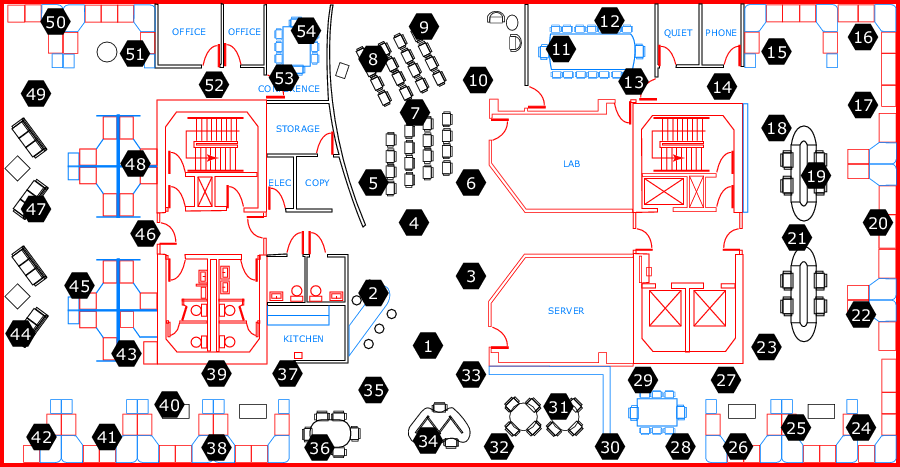
\includegraphics[width=0.7\linewidth]{figure/system/intel_sensor_dataset.png}
        \end{figure}
    \end{block}
\end{frame}

\begin{frame}{IoT Sensor Dataset Overview}
    \begin{block}{BTS Sensor Dataset}
        \begin{itemize}
            \item Collected timestamped temperature, humidity, frequency and voltage of power grid, motion, door, smoke, water leakage sensors, battery capacity, ...
            \item 4.2 million records
            \item Collection period: 2017
        \end{itemize}
        \begin{figure}
            \centering
            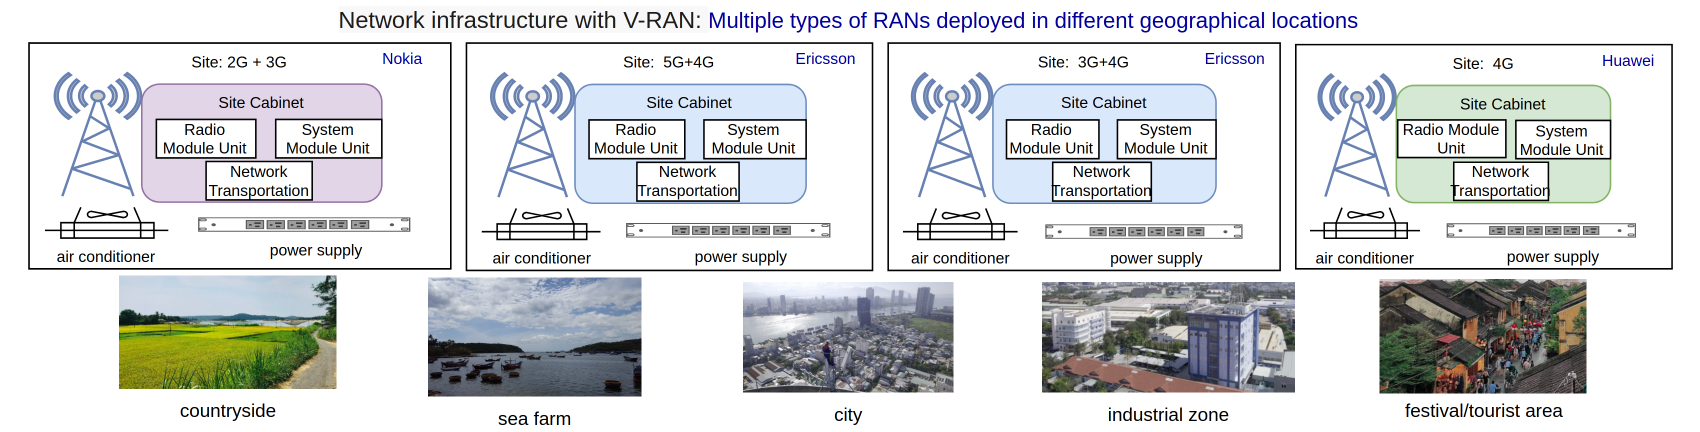
\includegraphics[width=\linewidth]{figure/system/bts_sensor.png}
        \end{figure}
    \end{block}
\end{frame}

\begin{frame}{IoT Sensor dataset overview}
    \begin{columns}
        \begin{column}{0.48\textwidth}
            \begin{figure}
                \centering
                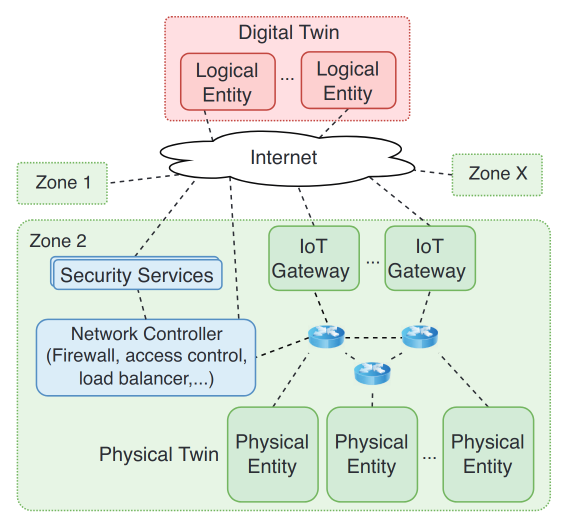
\includegraphics[width=\linewidth]{figure/related/sindit.png}
                \caption{Overview of a common deployment model for digital twin in manufacturing}
            \end{figure}
        \end{column}
        \begin{column}{0.48\textwidth}
            \begin{block}{SINDIT - Toy Factory Dataset}
                \begin{itemize}
                    \item SINDIT, a Digital Twin of the Fischertechnik Training Toy Factory
                    \item 37 sensors
                    \item Constantly send sensor data to the digital twin
                \end{itemize}
            \end{block}
            \begin{figure}
                \centering
                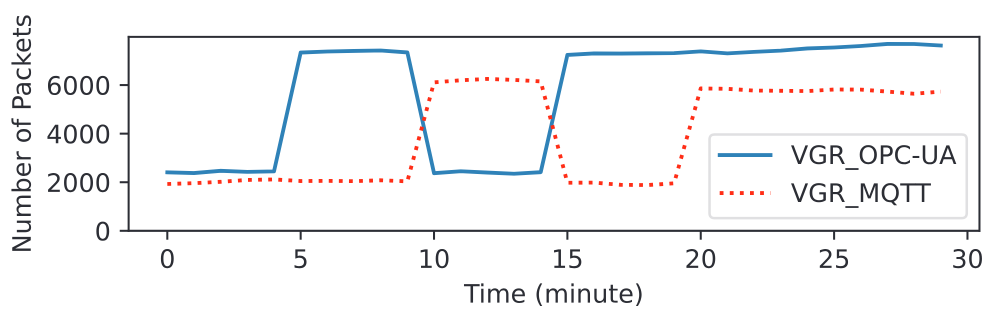
\includegraphics[width=\linewidth]{figure/related/vgr.png}
                \caption{Network packets from VGR (vision guided robot) to the two gateways.}
            \end{figure}
        \end{column}
    \end{columns}
    \footfullcite{nguyen2024security}
\end{frame}

\begin{frame}{IoT Sensor Dataset: Granularity}
    \begin{table}[h]
        \centering
        \caption{Summary interval between two events (in seconds)}
        \begin{tabular}{lrrrrrr}
            \toprule
            Dataset       & Number of sensors & Min      & Max        & Mean   & Std     & Median \\
            \midrule
            Berkeley      & 224       & 0.07     & 88198.38   & 61.72  & 555.04  & 35.24  \\
            BTS Sensor    & 1584      & 0.00     & 2954.00    & 51.54  & 214.58  & 18.00  \\
            Toy Factory    & 37        & 2.88     & 323335.69  & 8.87   & 1380.36 & 3.00   \\
            \bottomrule
        \end{tabular}
    \end{table}
\end{frame}

\begin{frame}{IoT Sensor Dataset: Autocorrelation}
    \begin{columns}
        \begin{column}{0.58\textwidth}
            \begin{figure}
                \centering
                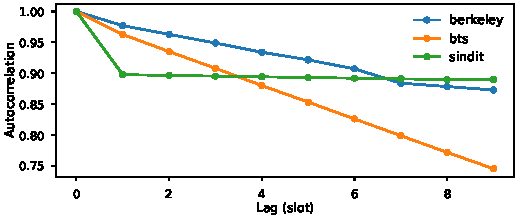
\includegraphics[width=\linewidth]{figure/system/plot_autocorr.pdf}
                \caption{Autocorrelation of time-series for each IoT dataset}
            \end{figure}
        \end{column}
        \begin{column}{0.38\textwidth}
            \begin{block}{Observation}
                \begin{itemize}
                    \item BTS: rich information
                    \item Berkeley: vary slower than BTS
                    \item SINDIT: abrupbt change in 1 time slot
                \end{itemize}
            \end{block}
        \end{column}
    \end{columns}
\end{frame}

\begin{frame}{AoII - Berkeley}
    \begin{columns}
        \begin{column}{0.48\textwidth}
            \begin{figure}
                \centering
                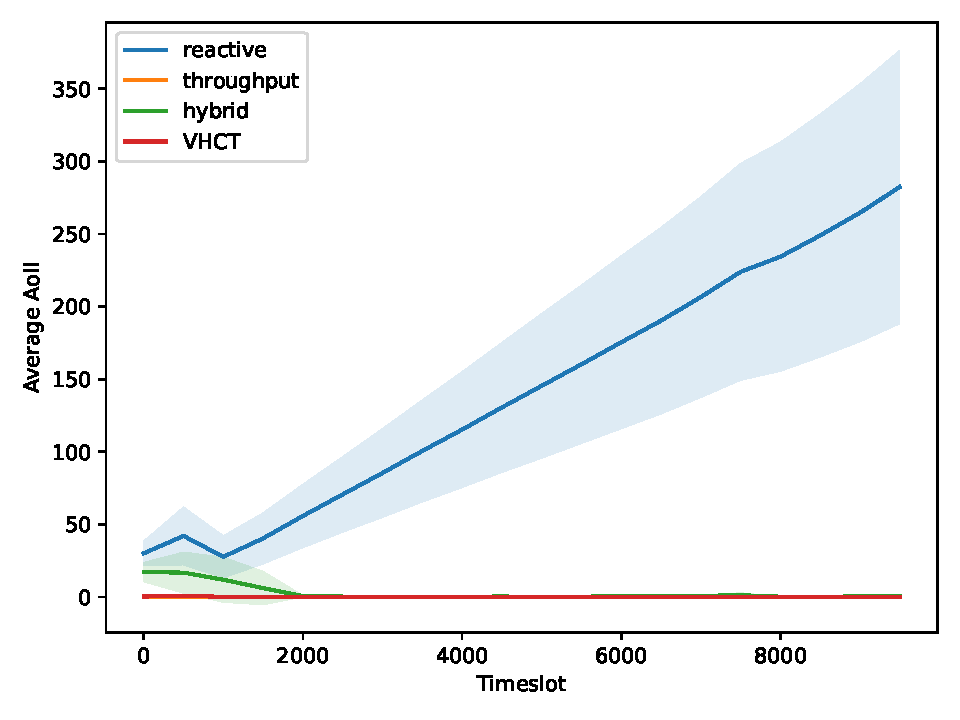
\includegraphics[width=\linewidth]{figure/simulation/plot_line_berkeley_avg_aoii_reactive_random_hybrid_vhct.pdf}
                \caption{Compare all sampling policies}
            \end{figure}
        \end{column}
        \begin{column}{0.48\textwidth}
            \begin{figure}
                \centering
                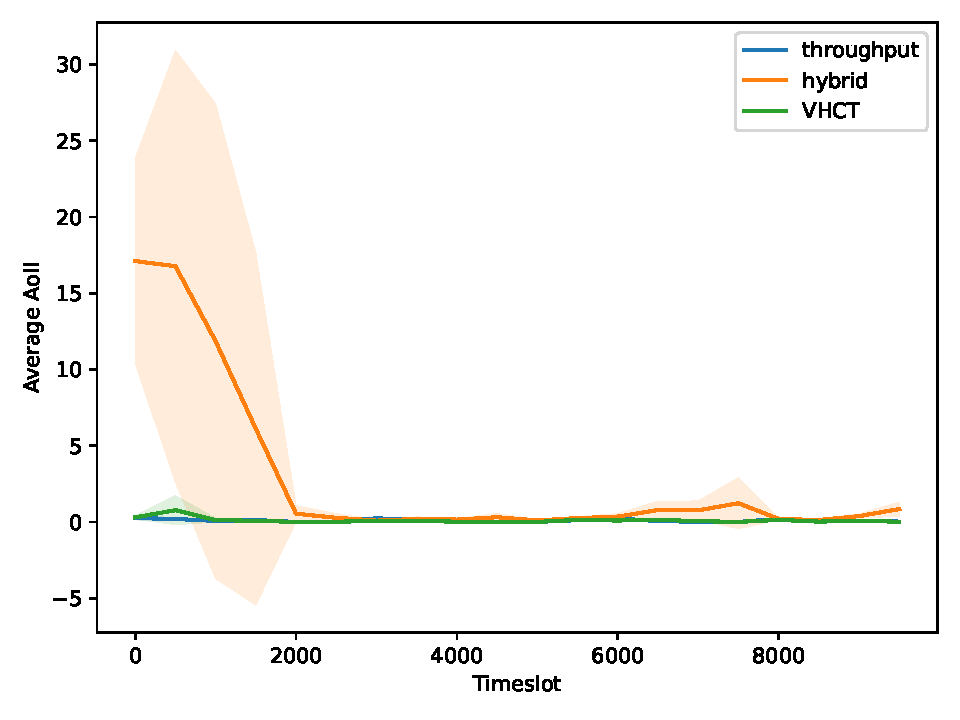
\includegraphics[width=\linewidth]{figure/simulation/plot_line_berkeley_avg_aoii_random_hybrid_vhct.pdf}
                \caption{Compare all sampling policies except reactive}
            \end{figure}
        \end{column}
    \end{columns}
\end{frame}

\begin{frame}{Channel Utilization - Berkeley}
    \begin{columns}
        \begin{column}{0.48\textwidth}
            \begin{figure}
                \centering
                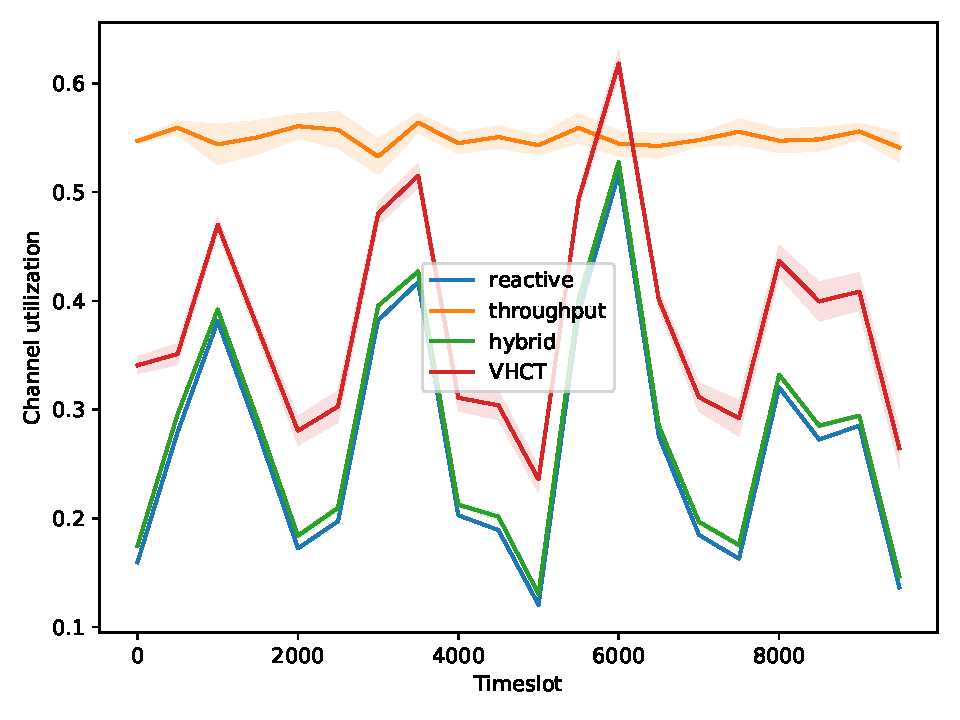
\includegraphics[width=\linewidth]{figure/simulation/plot_line_berkeley_utilization_reactive_random_hybrid_vhct.pdf}
                \caption{Compare all sampling policies}
            \end{figure}
        \end{column}
        \begin{column}{0.48\textwidth}
            \begin{figure}
                \centering
                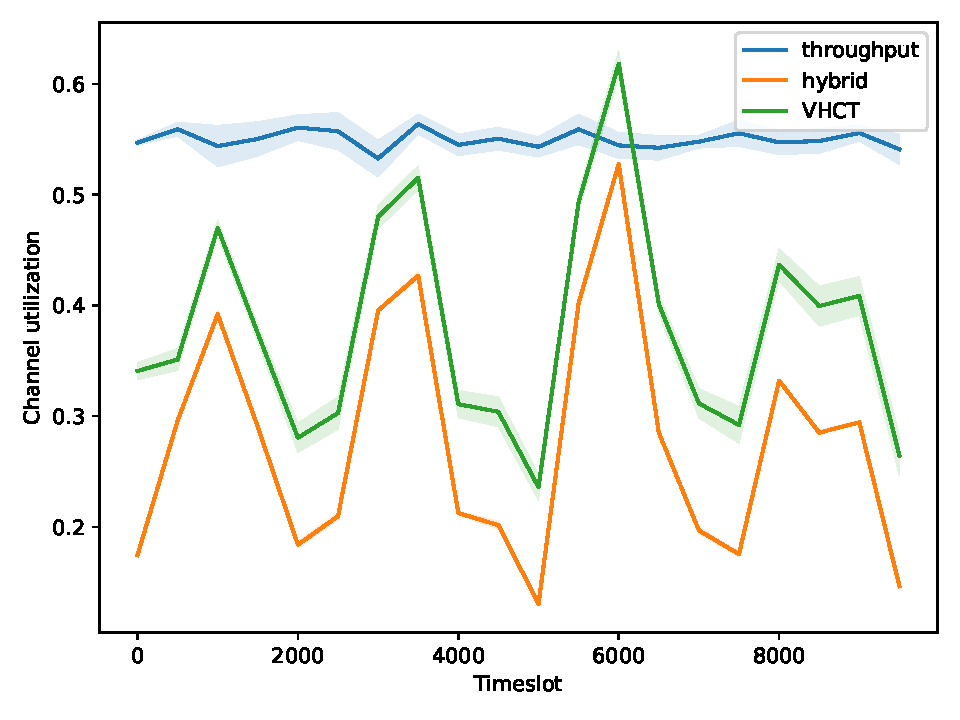
\includegraphics[width=\linewidth]{figure/simulation/plot_line_berkeley_utilization_random_hybrid_vhct.pdf}
                \caption{Compare all sampling policies except reactive}
            \end{figure}
        \end{column}
    \end{columns}
\end{frame}

\begin{frame}{Reward - Berkeley}
    \begin{columns}
        \begin{column}{0.48\textwidth}
            \begin{figure}
                \centering
                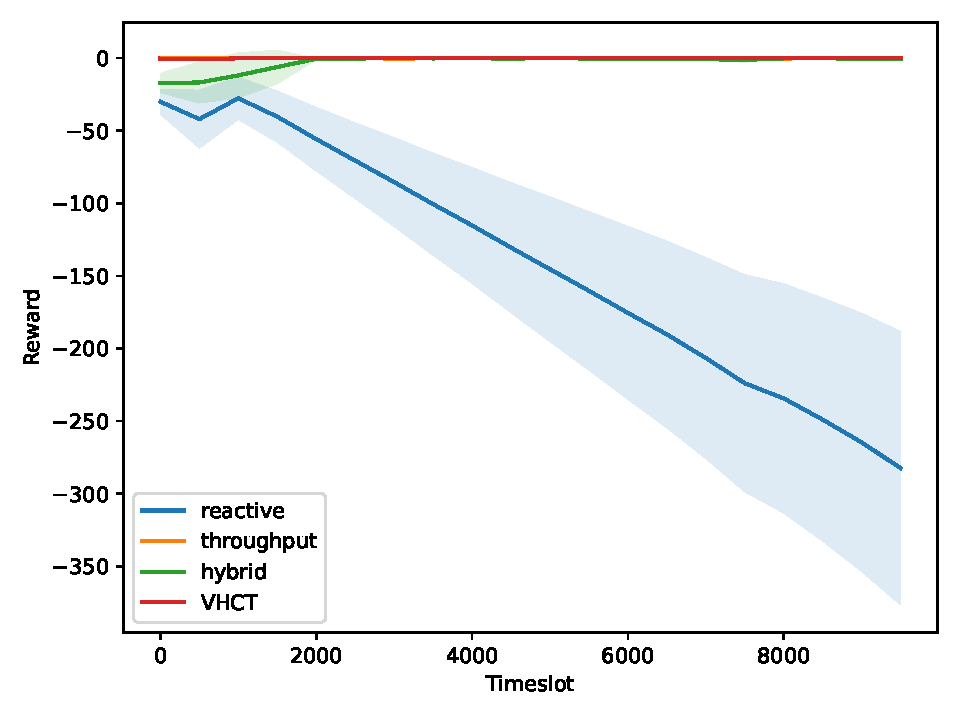
\includegraphics[width=\linewidth]{figure/simulation/plot_line_berkeley_reward_reactive_random_hybrid_vhct.pdf}
                \caption{Compare all sampling policies}
            \end{figure}
        \end{column}
        \begin{column}{0.48\textwidth}
            \begin{figure}
                \centering
                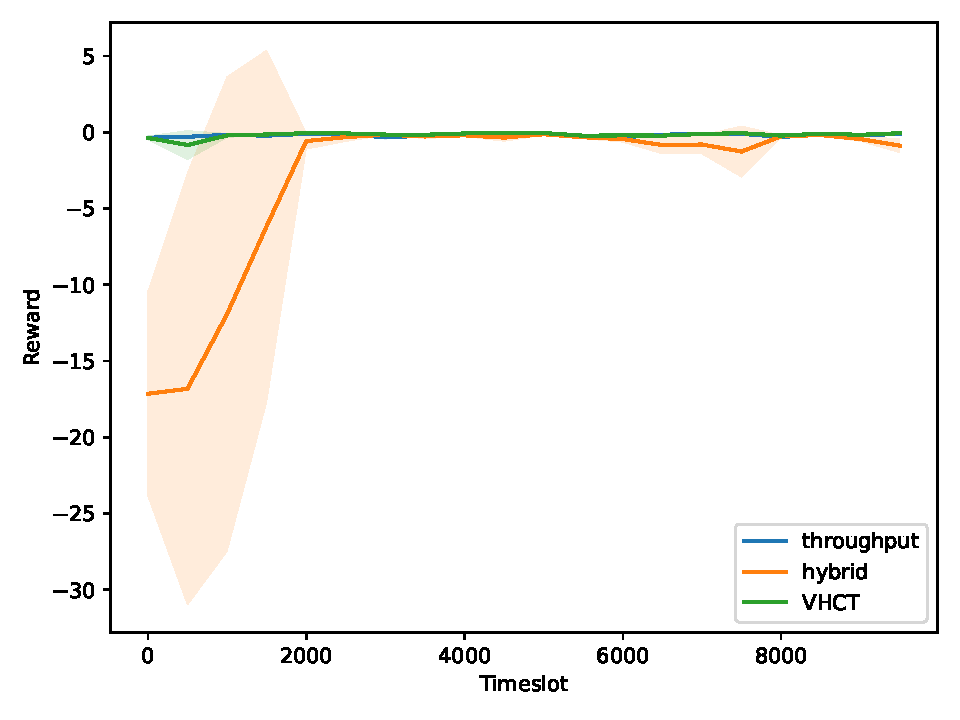
\includegraphics[width=\linewidth]{figure/simulation/plot_line_berkeley_reward_random_hybrid_vhct.pdf}
                \caption{Compare all sampling policies except reactive}
            \end{figure}
        \end{column}
    \end{columns}
\end{frame}

\begin{frame}{AoII - BTS}
    \begin{columns}
        \begin{column}{0.48\textwidth}
            \begin{figure}
                \centering
                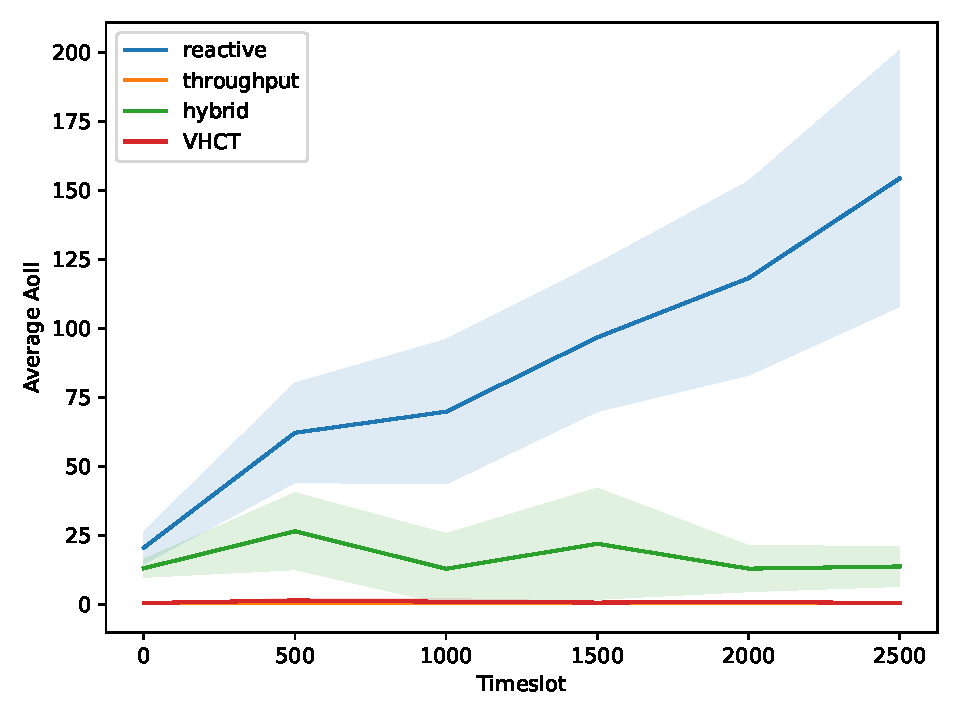
\includegraphics[width=\linewidth]{figure/simulation/plot_line_bts_avg_aoii_reactive_random_hybrid_vhct.pdf}
                \caption{Compare all sampling policies}
            \end{figure}
        \end{column}
        \begin{column}{0.48\textwidth}
            \begin{figure}
                \centering
                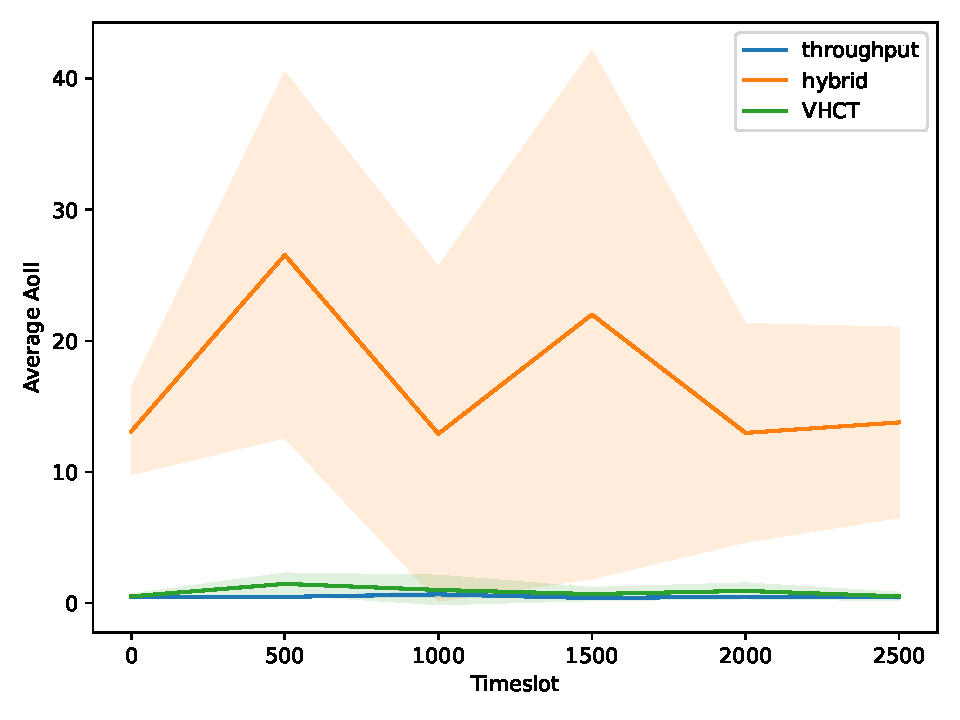
\includegraphics[width=\linewidth]{figure/simulation/plot_line_bts_avg_aoii_random_hybrid_vhct.pdf}
                \caption{Compare all sampling policies except reactive}
            \end{figure}
        \end{column}
    \end{columns}
\end{frame}

\begin{frame}{Channel Utilization - BTS}
    \begin{columns}
        \begin{column}{0.48\textwidth}
            \begin{figure}
                \centering
                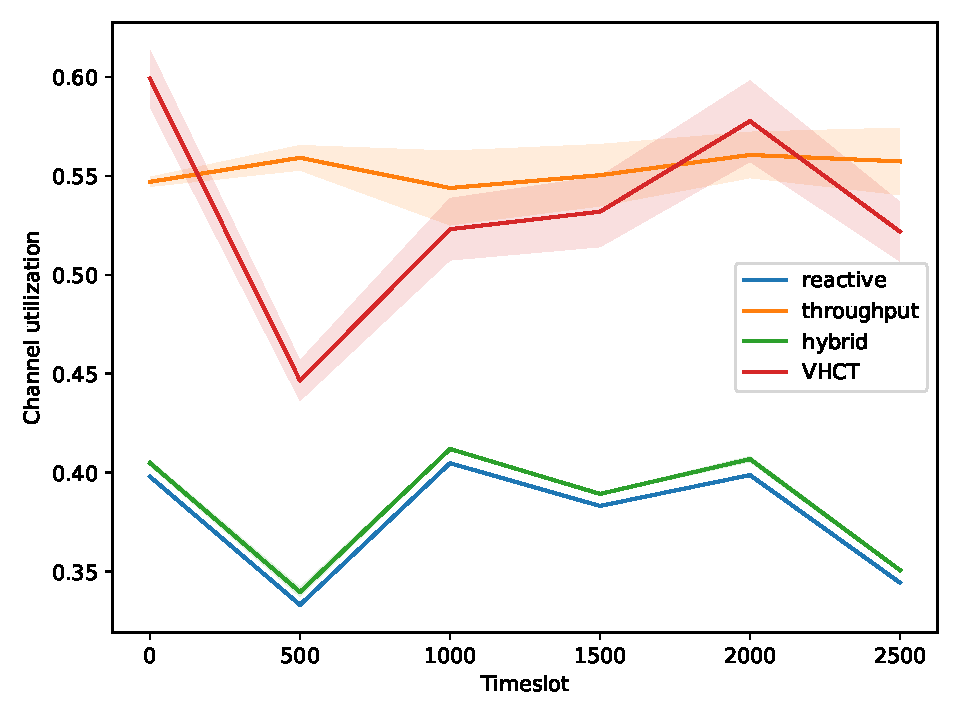
\includegraphics[width=\linewidth]{figure/simulation/plot_line_bts_utilization_reactive_random_hybrid_vhct.pdf}
                \caption{Compare all sampling policies}
            \end{figure}
        \end{column}
        \begin{column}{0.48\textwidth}
            \begin{figure}
                \centering
                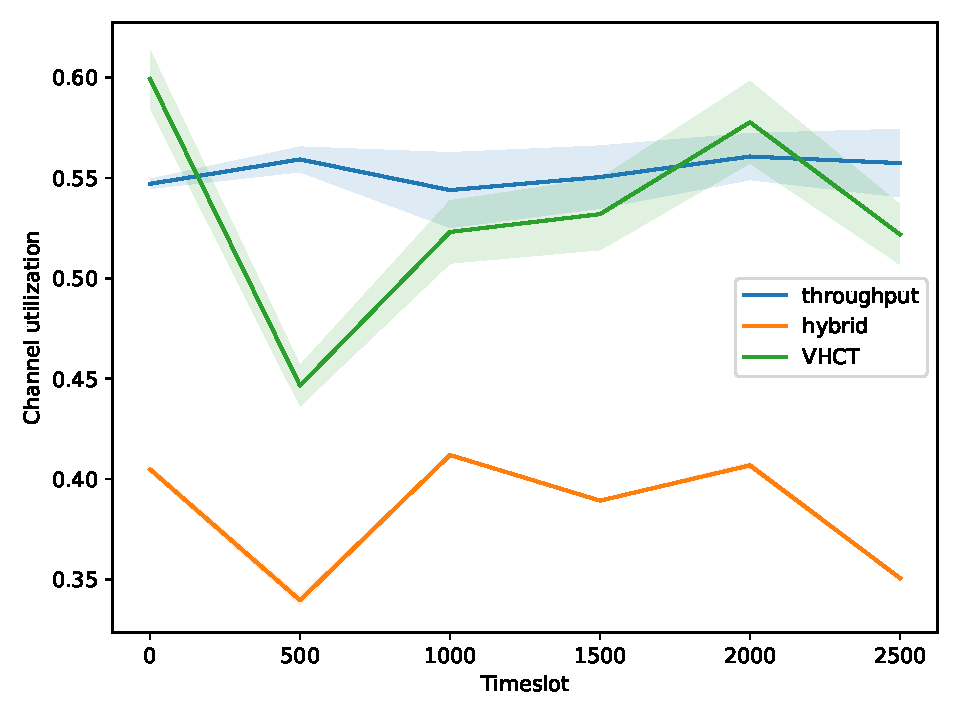
\includegraphics[width=\linewidth]{figure/simulation/plot_line_bts_utilization_random_hybrid_vhct.pdf}
                \caption{Compare all sampling policies except reactive}
            \end{figure}
        \end{column}
    \end{columns}
\end{frame}

\begin{frame}{Reward - BTS}
    \begin{columns}
        \begin{column}{0.48\textwidth}
            \begin{figure}
                \centering
                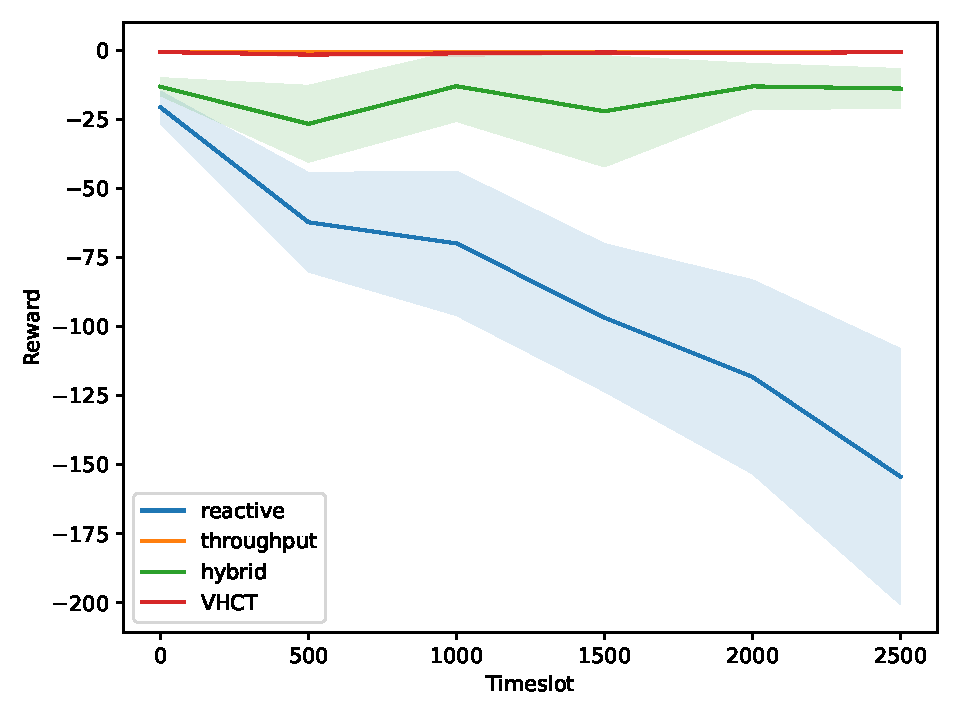
\includegraphics[width=\linewidth]{figure/simulation/plot_line_bts_reward_reactive_random_hybrid_vhct.pdf}
                \caption{Compare all sampling policies}
            \end{figure}
        \end{column}
        \begin{column}{0.48\textwidth}
            \begin{figure}
                \centering
                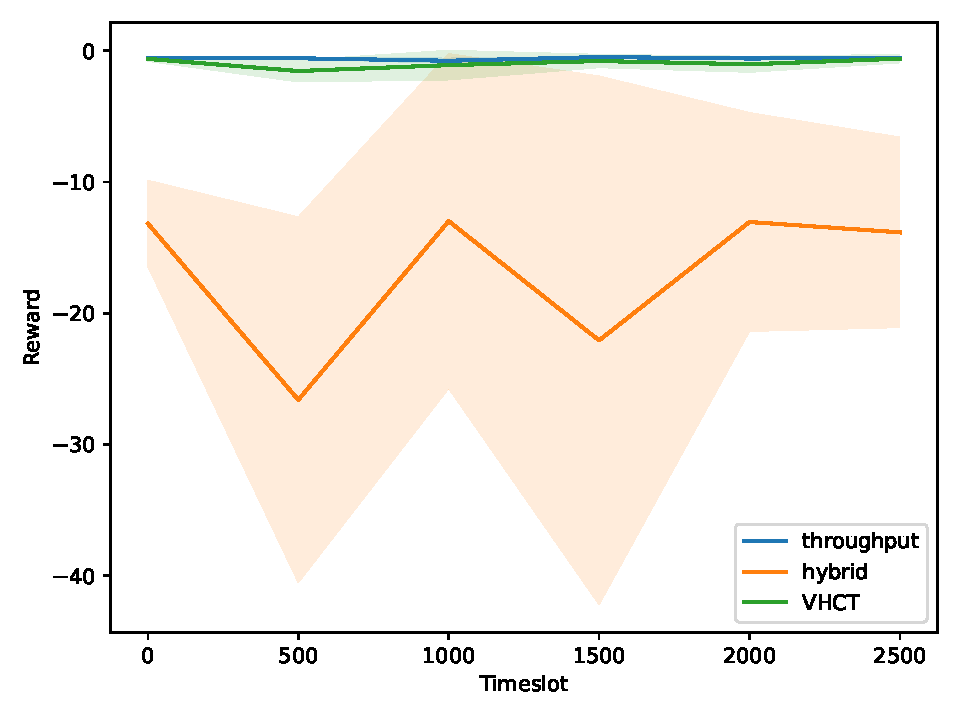
\includegraphics[width=\linewidth]{figure/simulation/plot_line_bts_reward_random_hybrid_vhct.pdf}
                \caption{Compare all sampling policies except reactive}
            \end{figure}
        \end{column}
    \end{columns}
\end{frame}

\begin{frame}{AoII - SINDIT}
    \begin{columns}
        \begin{column}{0.48\textwidth}
            \begin{figure}
                \centering
                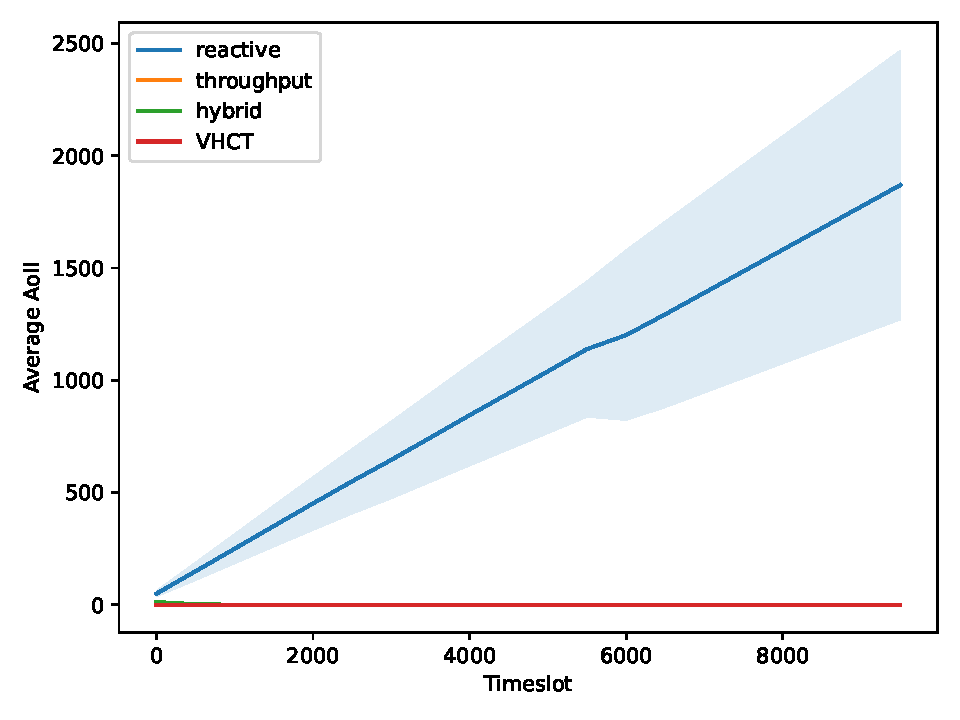
\includegraphics[width=\linewidth]{figure/simulation/plot_line_sindit_avg_aoii_reactive_random_hybrid_vhct.pdf}
                \caption{Compare all sampling policies}
            \end{figure}
        \end{column}
        \begin{column}{0.48\textwidth}
            \begin{figure}
                \centering
                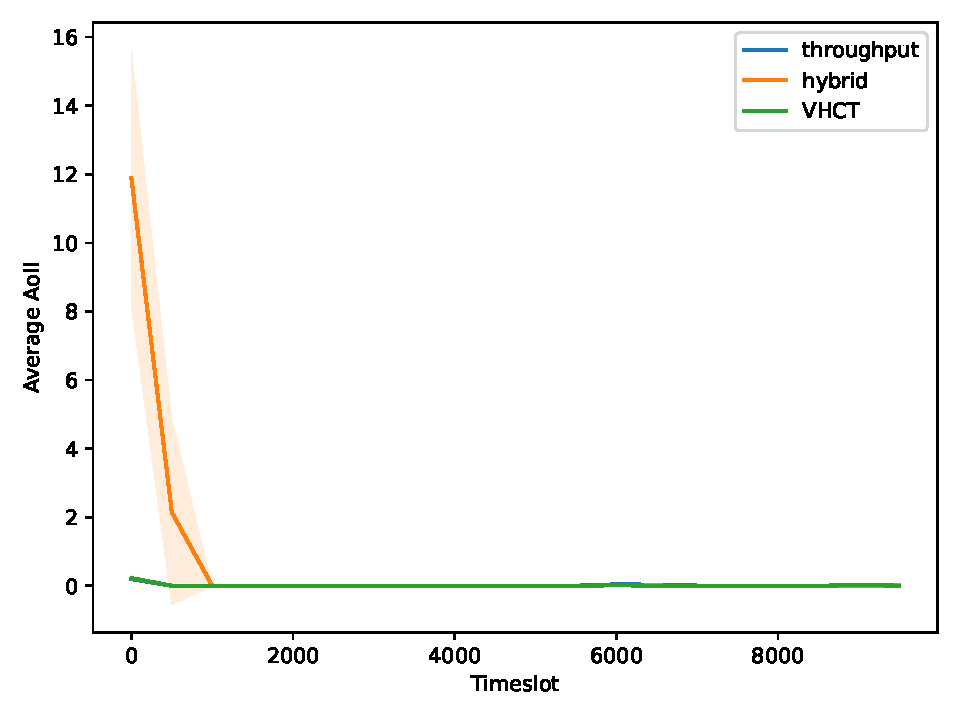
\includegraphics[width=\linewidth]{figure/simulation/plot_line_sindit_avg_aoii_random_hybrid_vhct.pdf}
                \caption{Compare all sampling policies except reactive}
            \end{figure}
        \end{column}
    \end{columns}
\end{frame}

\begin{frame}{Channel Utilization - SINDIT}
    \begin{columns}
        \begin{column}{0.48\textwidth}
            \begin{figure}
                \centering
                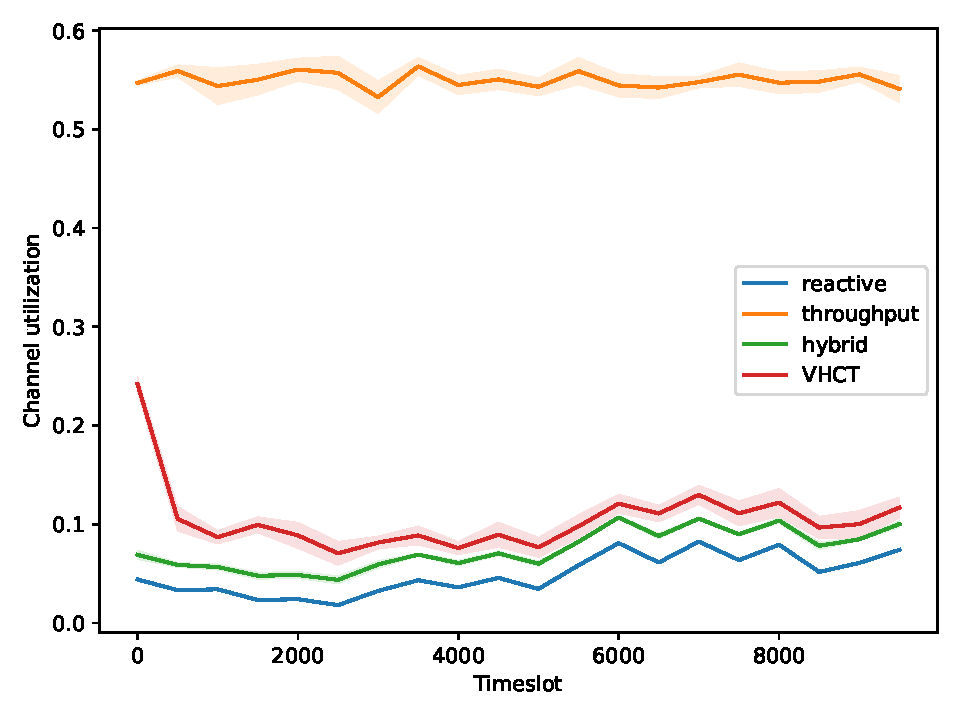
\includegraphics[width=\linewidth]{figure/simulation/plot_line_sindit_utilization_reactive_random_hybrid_vhct.pdf}
                \caption{Compare all sampling policies}
            \end{figure}
        \end{column}
        \begin{column}{0.48\textwidth}
            \begin{figure}
                \centering
                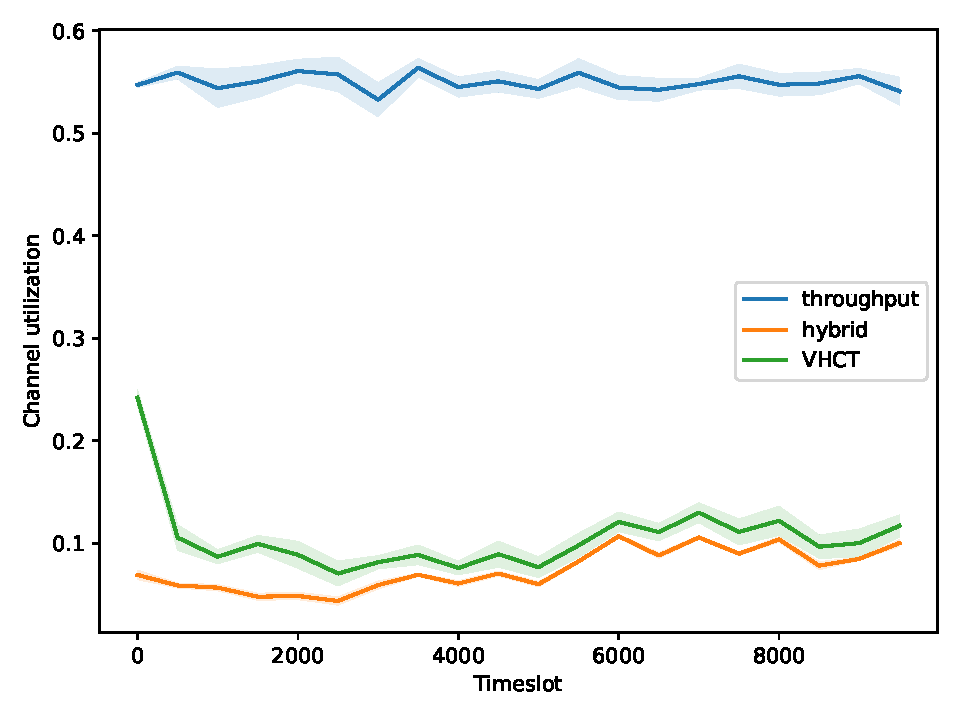
\includegraphics[width=\linewidth]{figure/simulation/plot_line_sindit_utilization_random_hybrid_vhct.pdf}
                \caption{Compare all sampling policies except reactive}
            \end{figure}
        \end{column}
    \end{columns}
\end{frame}

\begin{frame}{Reward - SINDIT}
    \begin{columns}
        \begin{column}{0.48\textwidth}
            \begin{figure}
                \centering
                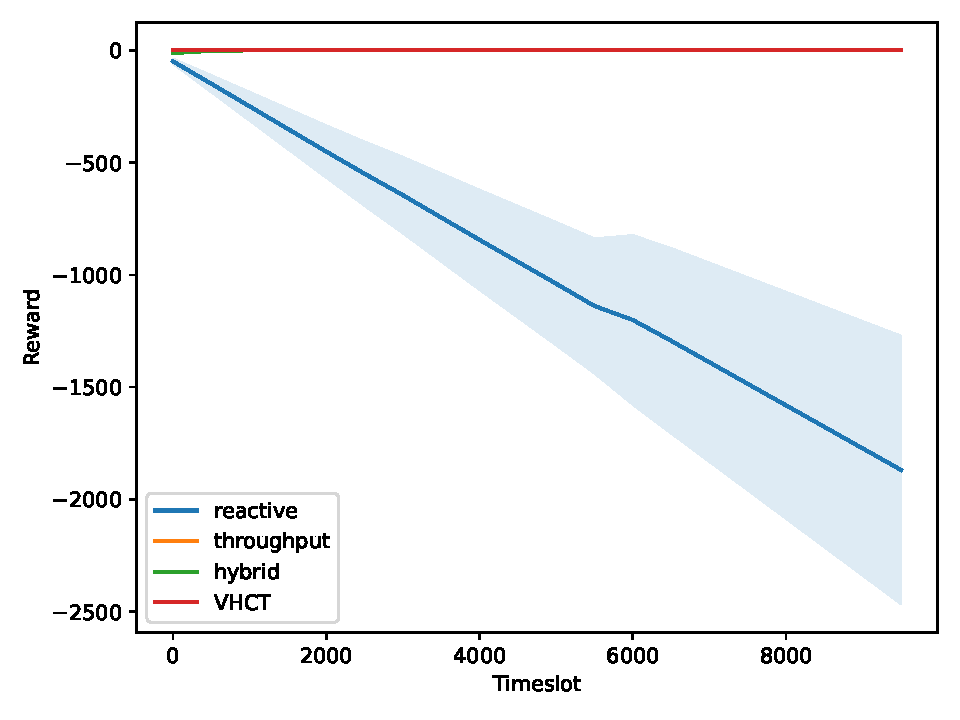
\includegraphics[width=\linewidth]{figure/simulation/plot_line_sindit_reward_reactive_random_hybrid_vhct.pdf}
                \caption{Compare all sampling policies}
            \end{figure}
        \end{column}
        \begin{column}{0.48\textwidth}
            \begin{figure}
                \centering
                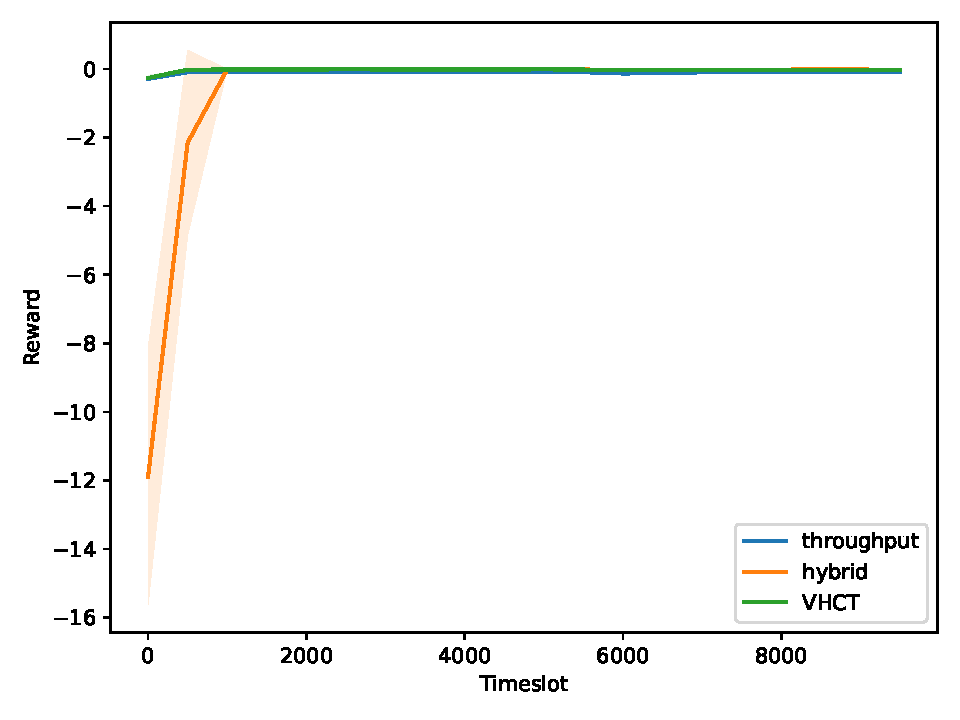
\includegraphics[width=\linewidth]{figure/simulation/plot_line_sindit_reward_random_hybrid_vhct.pdf}
                \caption{Compare all sampling policies except reactive}
            \end{figure}
        \end{column}
    \end{columns}
\end{frame}

\begin{frame}{VHCT's performance on different datasets}
    \begin{columns}
        \begin{column}{0.48\textwidth}
            \begin{figure}
                \centering
                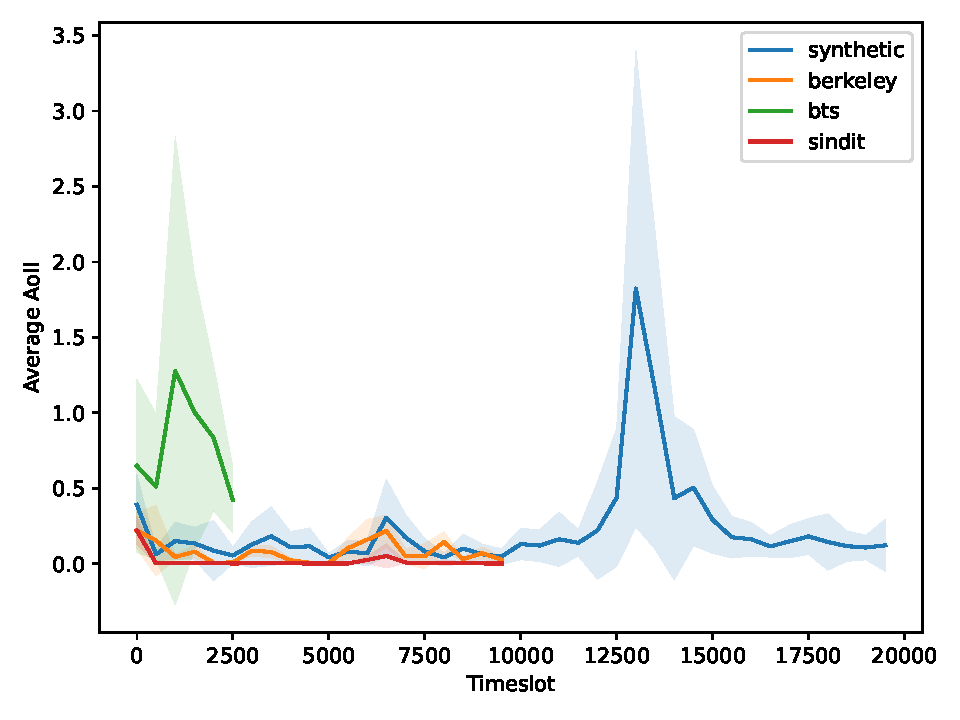
\includegraphics[width=\linewidth]{figure/simulation/plot_line_v2_vhct_avg_aoii.pdf}
                \caption{Avg AoII}
            \end{figure}
        \end{column}
        \begin{column}{0.48\textwidth}
            \begin{figure}
                \centering
                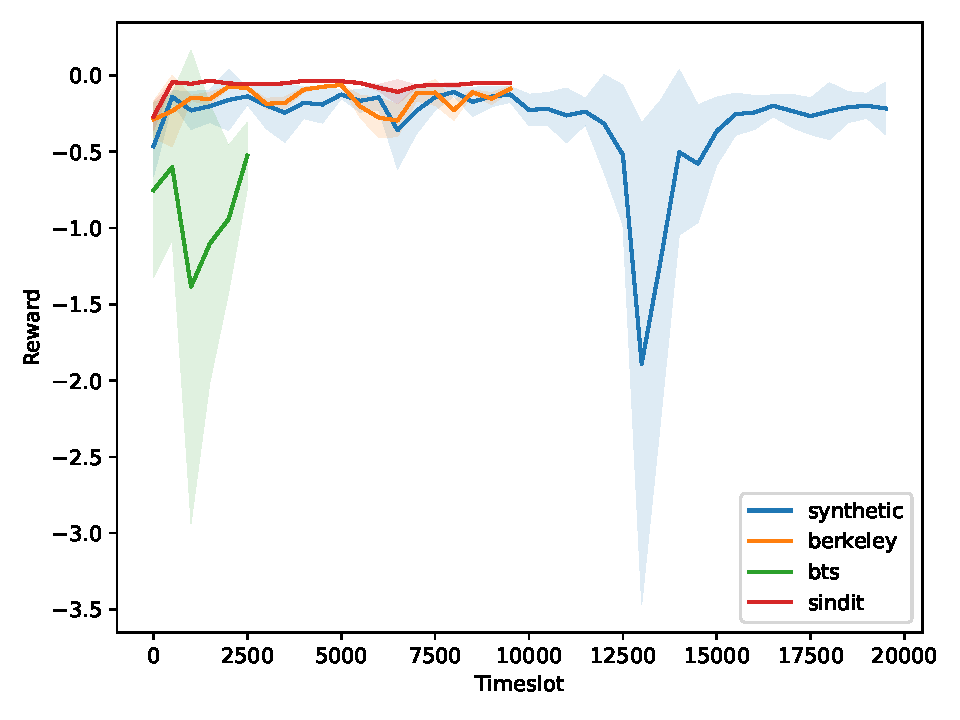
\includegraphics[width=\linewidth]{figure/simulation/plot_line_v2_vhct_reward.pdf}
                \caption{Reward}
            \end{figure}
        \end{column}
    \end{columns}
\end{frame}

\subsection*{Conclusion}

\begin{frame}{Conclusion}
    \begin{block}{Summary}
        \begin{itemize}
            \item Apply VHCT, a \gls{xab} algorithm for \alert{online batch learning} to select best sampling rate
            \item Measure \alert{end-to-end performance} on modern grant-free random access (\gls{irsa} model)
            \item Test on AaltoSEA's \alert{realistic IoT dataset} (faster fluctuation in data $rightarrow$ more demand)
            \item Minimize \alert{\gls{aoii}} while sending data \alert{conservatively}, compared to heuristic baselines
        \end{itemize}
    \end{block}
    \begin{block}{Acknowledgement}
        This work was supported in part by JST ASPIRE under Grant JPMJAP2325
    \end{block}
\end{frame}

\begin{frame}{Activities}
    \begin{figure}
        \centering
        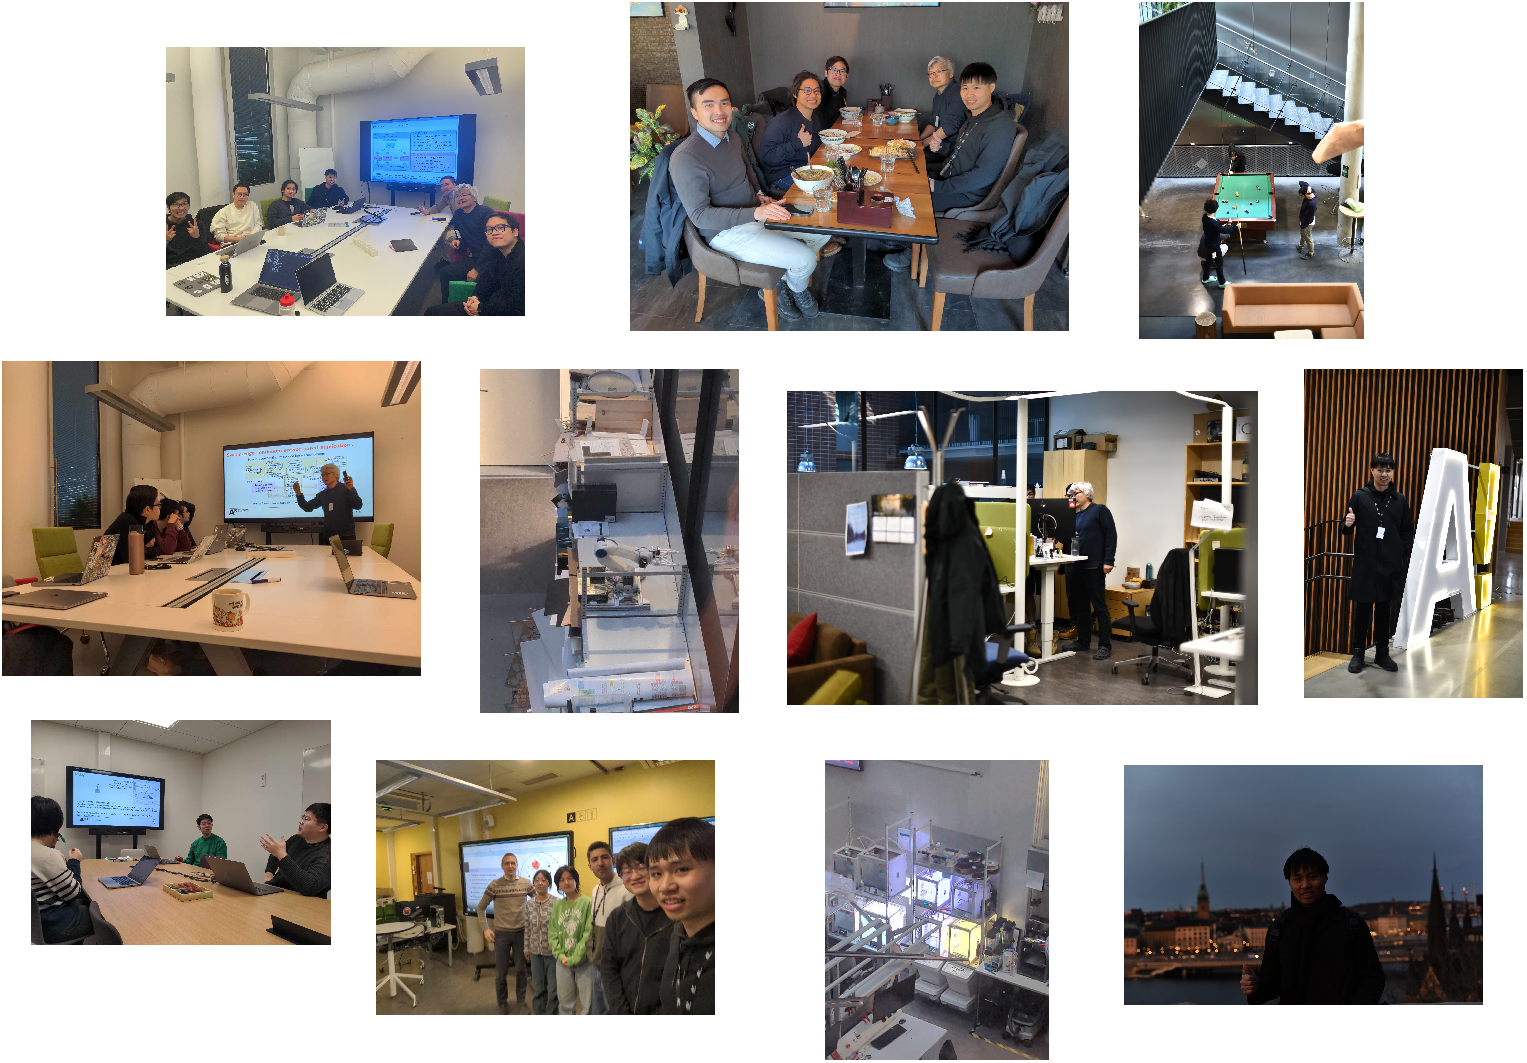
\includegraphics[width=0.9\linewidth]{figure/conclusion/aoii-iot-data-activities.pdf}
    \end{figure}
\end{frame}
\end{document}
